\documentclass{beamer}
\usepackage{caption}
\usepackage{subcaption}
\usepackage{slashed}
\usepackage{tikz}
\usetheme{Luebeck}
\setbeamertemplate{navigation symbols}{}
\setlength{\parskip}{2.5mm}
\title[Searching for Dilepton SUSY with $t\bar{t}$ backgrounds\hspace{2.5em}\insertframenumber/18]{Searching for Supersymmetry in the Dilepton channel with large top quark backgrounds} %with $t \bar{t}$ background estimation\hspace{14em}\insertframenumber/17]{Di-lepton $t \bar{t}$ estimation from \\ Semi-leptonic $t \bar{t}$}
%\author{\emph{Tim Brooks}, Glen Cowan, Aftab Alam}
\author{\emph{Tim Brooks}, Glen Cowan}
\institute{Royal Holloway University of London}
\date{17/4/13}
\begin{document}

\begin{frame}
\titlepage
\end{frame}

\section{Search}
\begin{frame}{Search for Supersymmetry}
  \begin{itemize}
    \item Supersymmetry predicts new particles accessable in high energy proton-proton collisions such as at the LHC
    \item SUSY particle decays can give final states with leptons jets and missing energy
    \item $E_{T}^{miss}$ is a powerful discriminator for R-parity preserving SUSY models
    \item A Di-lepton selection is powerful in detecting a class of models with weak gaugino and/or slepton production
  \end{itemize}
$\Rightarrow$ Search for Supersymmetry in the $2 \text{lepton} + E_{T}^{\text{miss}} + \text{jets}$ channel.
\end{frame}

\begin{frame}{Dilepton SUSY event}
  \begin{figure}
    \centering
    %\def\svgwidth{\columnwidth}
    \includegraphics[scale=5.0]{img/susy.pdf}
  \end{figure}
\end{frame}

\begin{frame}{Dilepton SUSY search}
\begin{itemize}
    \item Additional jets in events also give power when decay cascades have large mass gaps between SUSY particles

    \item Length of cascade determines the number of jets. Most searches looks for 2 or 3 hard jets in addition to the leptons + $E_{T}^{miss}$.

    \item The largest background to these searches is usually top pair production, $t\bar{t}$.
\end{itemize}
\end{frame}

%\begin{frame}{Backgrounds}
%Several standard model processes produce similar multi-object states:
%
%\begin{table}
%\centering
%\begin{tabular}{l||c|c}
%                     & Real leptons               & Fake leptons         \\
%\hline \hline
%Real $\slashed{E}_{T}$ & $t\bar{t}$, Diboson + jets & W + jets, Single top \\
%\hline
%Fake $\slashed{E}_{T}$ & Z + jets                   & W + jets, QCD        \\
%\end{tabular}
%%\caption{This table shows some data}
%\label{tab:myfirsttable}
%\end{table}
%
%$t\bar{t}$ is normally the largest background.
%\end{frame}

\section{Control sample}

\begin{frame}{Dileptonic $t\bar{t}$}
  \begin{figure}
    \centering
    Production and decay of $t\bar{t}$ via b-jets and leptonically decaying W-bosons.
    \includegraphics[scale=8.0]{img/dl-ttbar.pdf}
  \end{figure}
\end{frame}

\begin{frame}{Backgrounds}
Need to estimate dilepton $t\bar{t}$ in search region. Monte Carlo techniques are limited by theoretical uncertainty. Current approaches tag dilepton $t\bar{t}$ in data using known properties of decay.

Our approach - measure $t\bar{t}$ in the semi-leptonic channel and swap $W\rightarrow jj$ for $W\rightarrow l\nu$. Dressed control sample reflects kinematic properties of dileptonic $t\bar{t}$ and may be selected with the search criteria.

Only rely upon MC for a scale factor, $\tau$, relating true dilepton $t\bar{t}$ to our control sample in the signal region.
\end{frame}

\begin{frame}{Semileptonic $t\bar{t}$}
  \begin{figure}
    \centering
    More commonly, one W-boson decays hadronically.
    \includegraphics[scale=6.0]{img/sl-ttbar.pdf}
  \end{figure}
\end{frame}

\begin{frame}{Control method}
Our method outline is as follows:
  \begin{itemize}
    \item Select a sample of $t \bar{t}$ by selecting events with 1 lepton, missing $E_{t}$ and at least 4 jets.
    \item Reconstruct each event to replace jets from hadronic W decay with a simulated lepton-neutrino pair.
    \item Accept events that are compatible with well reconstructed $t \bar{t}$
    \item Use resulting sample to predict dilepton $t \bar{t}$ events passing signal selection.
    \item Apply a scale factor from Monte Carlo to estimate the total number of events in the signal region from $t \bar{t}$.
  \end{itemize}
\end{frame}

\begin{frame}{Reconstruction}
  \begin{figure}
    \centering
    %\def\svgwidth{\columnwidth}
    \includegraphics[scale=0.3]{img/drawing.pdf}
  \end{figure}
  Association between the truth partons of a $t \bar{t}$ event and the reco-level jets in a candidate event are described by a map: $\left(q1:a, q2:b, b1:c, b2:d\right)$.

  For 4 jets there are 24-unique mappings. To reconstruct the neutrino momenta, we use constraints of the $t \bar{t}$ system. This gives a sign ambiguity leading to 48 combinations.%The number of maps does not grow as the factorial of the number of jets, since we only consider those that are unique in their first 4 assignments.
\end{frame}

% \begin{frame}{Reconstruction}
%   In the majority of dilepton top-events, there are 4 truth partons of interest:
%   \begin{itemize}
%     \item A u-d or c-s quark pair from a top - via a W-boson: $q_{1}$,$q_{2}$.
%     \item A b quark produced in association with the hadronic W: $b_{1}$.
%     \item A b quark produced in association with the leptonic W: $b_{2}$.
%   \end{itemize}
%   Association between the truth partons of a $t \bar{t}$ event and the reco-level jets in a candidate event are described by a map: $\left(q1:a, q2:b, b1:c, b2:d\right)$.

%   For 4 jets there are 24-unique mappings. To reconstruct the neutrino momenta, we use constraints of the $t \bar{t}$ system. This gives a sign ambiguity leading to 48 combinations.%The number of maps does not grow as the factorial of the number of jets, since we only consider those that are unique in their first 4 assignments.
% \end{frame}

\begin{frame}{Reconstruction}
Select $t\bar{t}$ using a $\chi^2$ with knowledge of the top system-

\begin{equation*}\begin{split}
  \chi^2 &= \frac{\left(M_{ab} - M_W\right)^2}{\sigma^2_{M_{W_h}}} + \frac{\left(M_{abc} - M_t\right)^2}{\sigma^2_{M_{t_h}}} + \frac{\left(M_{dl\nu} - M_t\right)^2}{\sigma^2_{M_{t_l}}} \\
  &-2\ln{\frac{L_{W}\left( \omega_{a},\omega_{b} \right)}{f^{\text{max}}_{a} f^{\text{max}}_{b}}} -2\ln{\frac{f\left(\omega_{c} \big| b\right)}{f^{\text{max}}_{c}}} -2\ln{\frac{f\left(\omega_{d} \big| b\right)}{f^{\text{max}}_{d}}}
\end{split}\end{equation*}
With $f^{\text{max}}_j = \max\left[f\left(\omega_{j} \big| l\right), f\left(\omega_{j} \big| c\right), f\left(\omega_{j} \big| b\right)\right]$

$f\left( \omega_{j} \big| F\right)$ is a Kernal Density Estimator parameterising the b-tagger response to flavour $F$ evaluated with the weight from jet $j$.
\end{frame}

\begin{frame}{KDE parameterisation}
  \begin{columns}
    \begin{column}{0.5\textwidth}\begin{figure}
      % \caption{b-tag distributions}
      \centering
      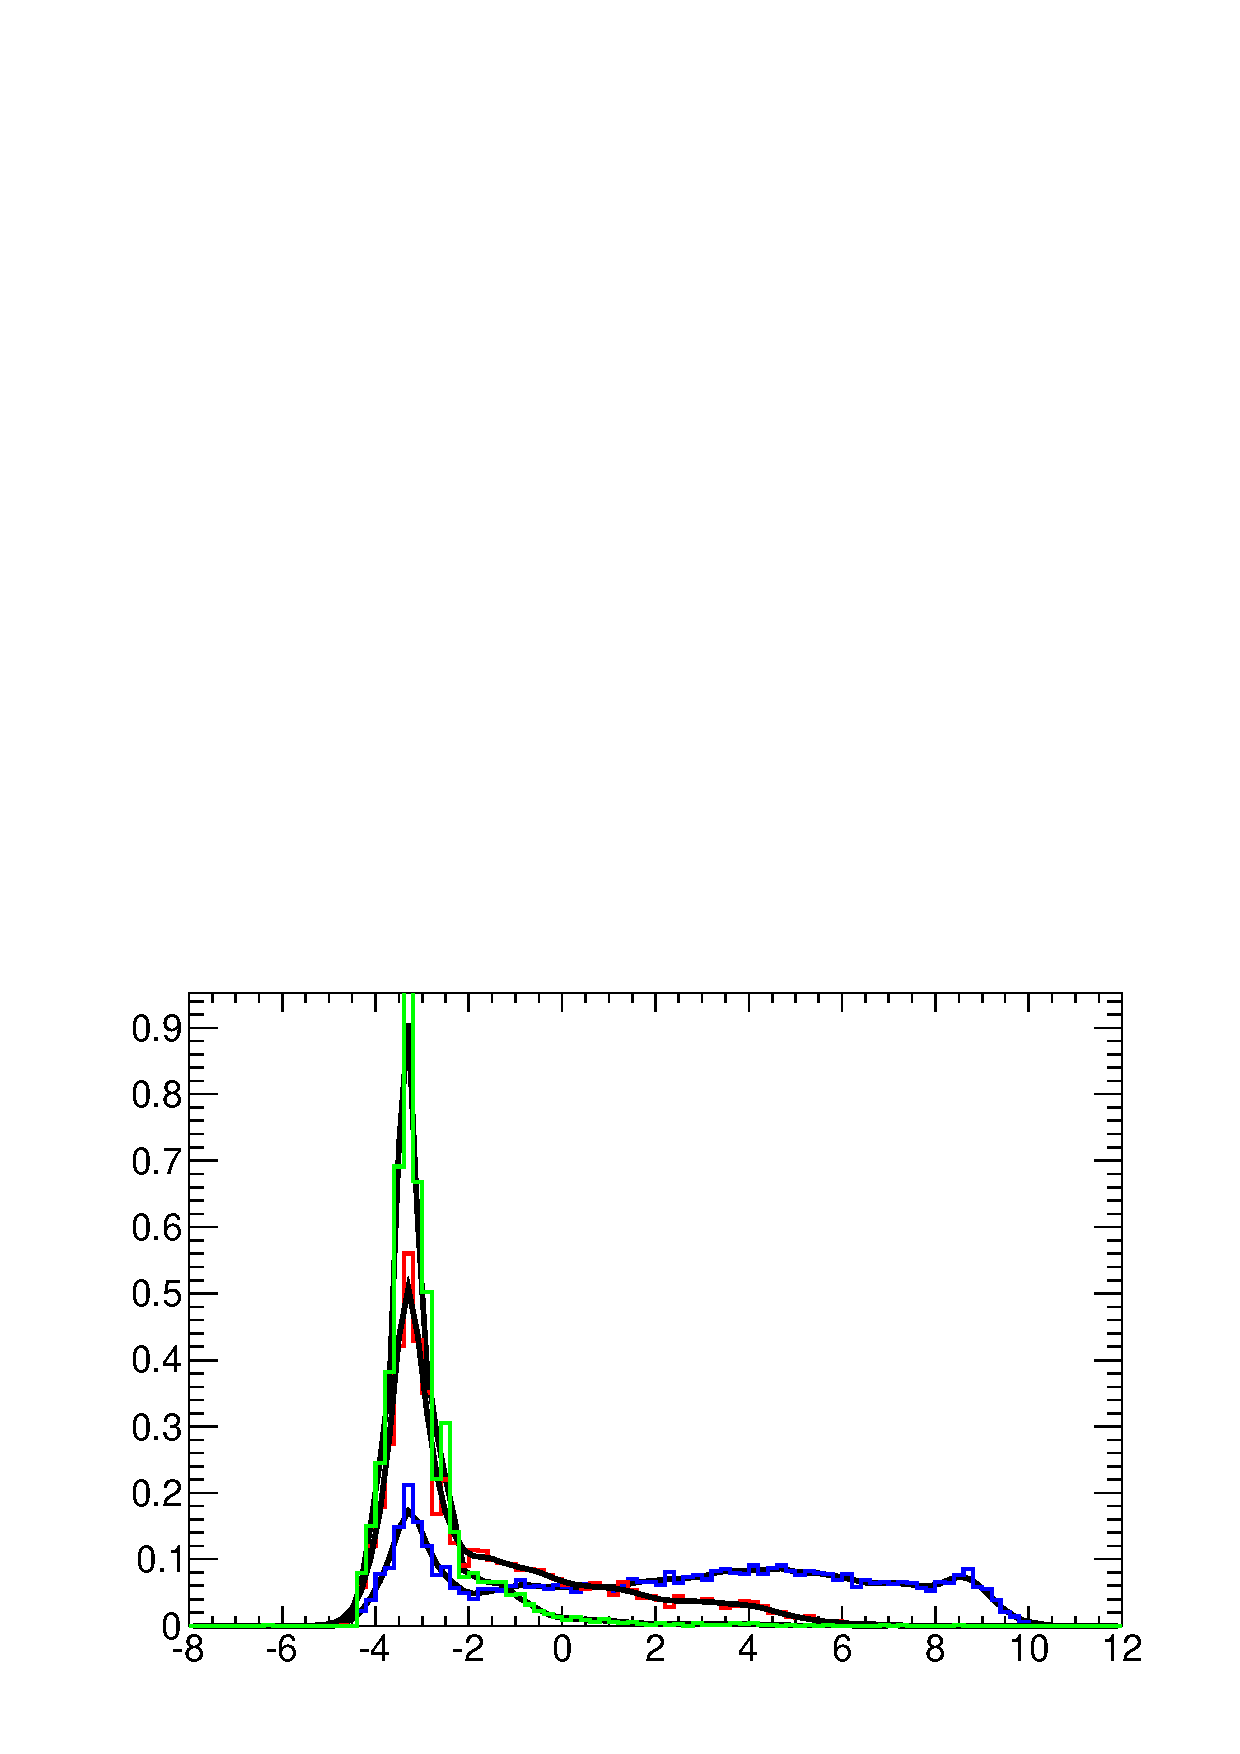
\includegraphics[scale=0.3]{img/tagging.pdf}
      % Classifier output
    \end{figure}\end{column}
    \begin{column}{0.5\textwidth}\begin{figure}
        % KDEs parameterise b-jet response
    %   % \caption{b-tag distributions}
       \includegraphics[scale=0.3]{img/jets.pdf}
    \end{figure}\end{column}
  \end{columns}
\end{frame}

\begin{frame}{Total Chisquare distribution}
  \begin{columns}
    \begin{column}{0.5\textwidth}\begin{figure}
      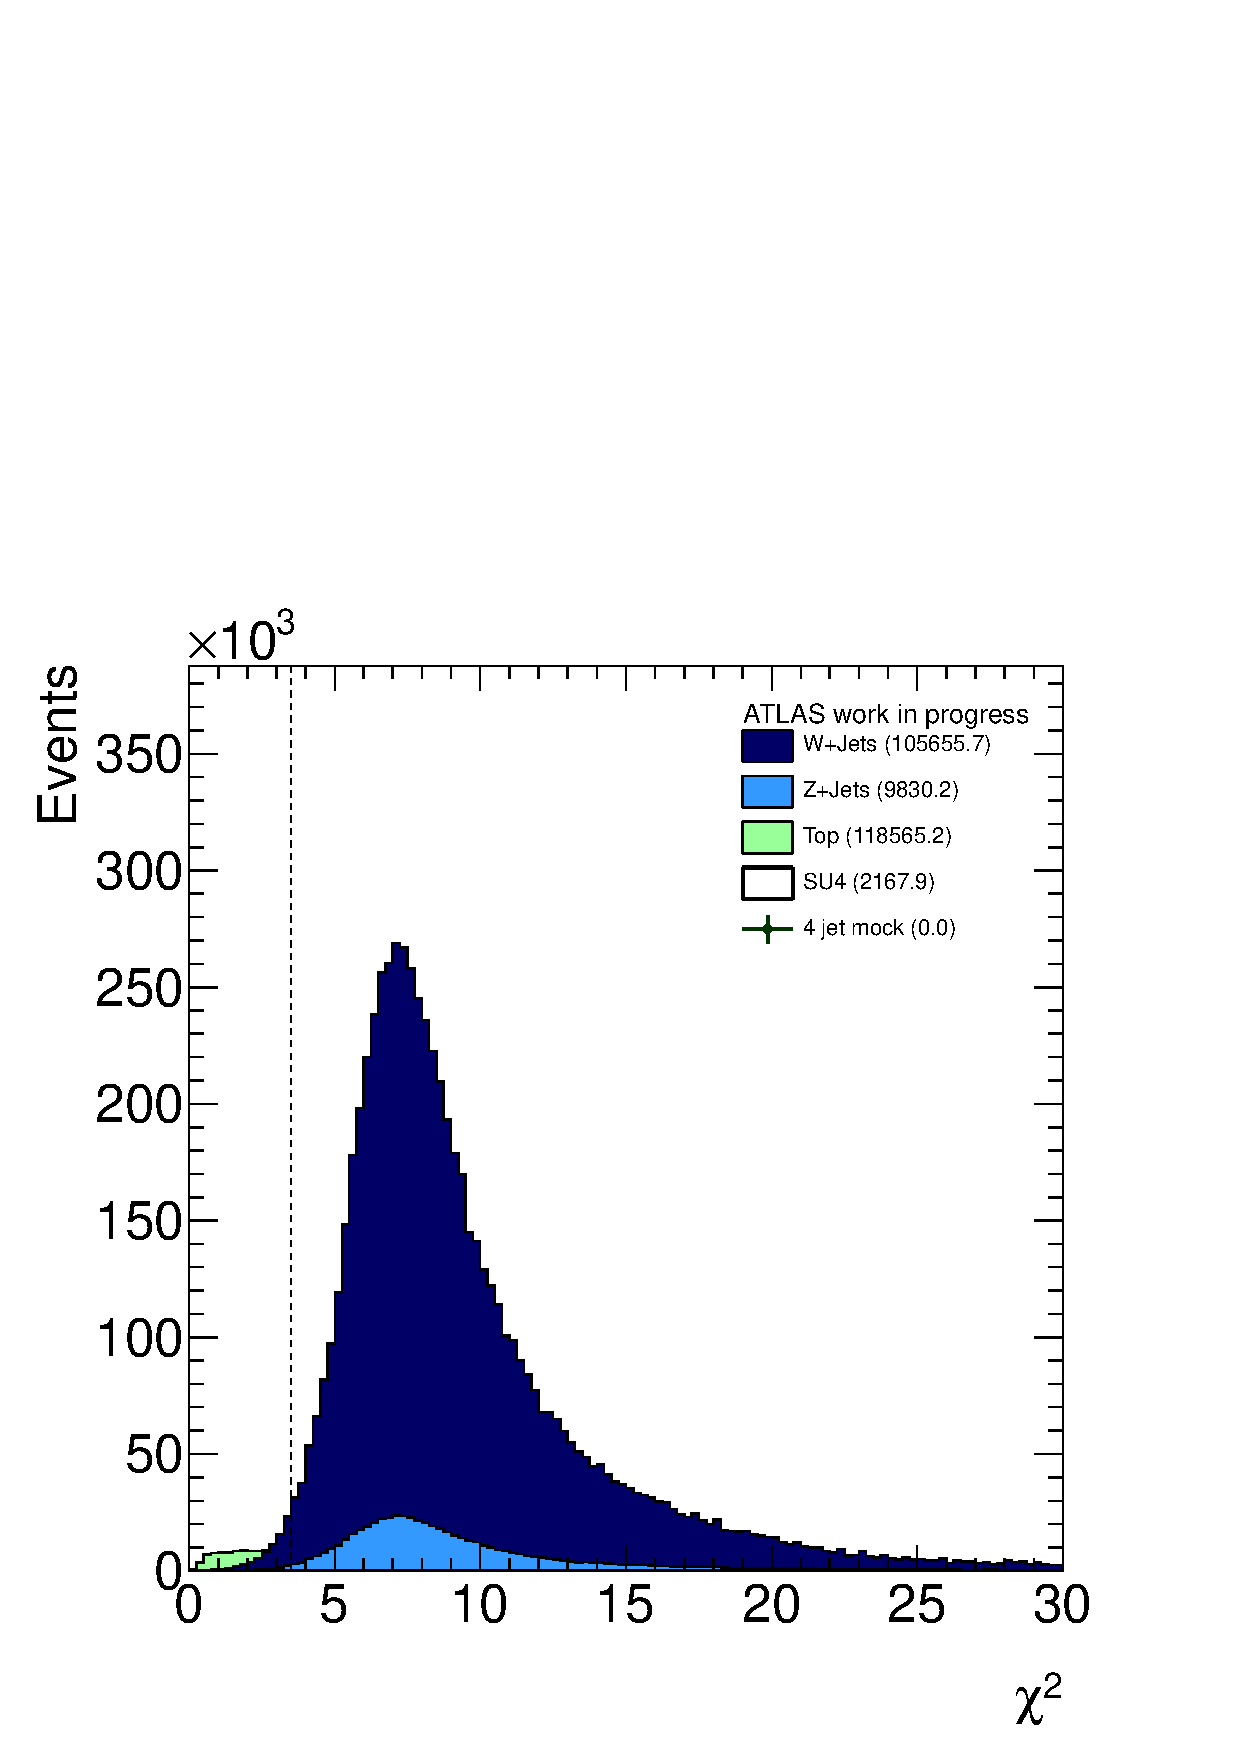
\includegraphics[scale=0.325]{img/Total__min_chi_all_all4.pdf}
      % \caption{$\chi^2$ = $\chi^2_{kinematic} + \chi^2_{B}$}
    \end{figure}\end{column}
  \end{columns}
\end{frame}

\begin{frame}%{Significance measure}
Two measurements from data; events in signal selection, $n$ and events in control selection, $m$.

Model measurements as Poisson distributed with expectations;
\begin{eqnarray*}
    E[n] = \mu s + b_{t\bar{t}} + b_{o}^{SR} \\*[0.2 cm]
    E[m] = \mu s' + \tau b_{t\bar{t}} + b_{o}^{CR}
\end{eqnarray*} \\
% with signal strength parameter, $\mu$,

%     events from signal process in signal selection, $s$ and in control selection, $s'$

%     events from $t\bar{t}$ background in signal selection, $b_{t\bar{t}}$ and signal-control ratio, $\tau$

%     events from other backgrounds in signal selection, $b_{o}^{SR}$ and signal-control ratio, $b_{o}^{CR}$
where; \\
 \begin{tabular}{r l}
     $\mu$ & signal strength parameter \\
     $s$ & predicted signal events in signal region \\
     $b_{t\bar{t}}$ & $t\bar{t}$ background events in signal region \\
     $b_{o}^{SR}$ & predicted events from other backgrounds in signal region \\
     $s'$ & predicted signal events in control region \\
     $\tau$ & ratio of $t\bar{t}$ events in signal region to control region \\
     $b_{o}^{CR}$ & events from other backgrounds in control region
 \end{tabular}

\end{frame}

\begin{frame}
With $\zeta = log\left(\tau\right)$, $\beta_{o} = log\left(b_{o}^{CR}\right)$, and the predicted values $\tilde{\zeta}$, $\tilde{\beta_{o}}$;
% With predicted $\tau$, $\tilde{\tau}$ and predicted $b_{o}^{CR}$, $\tilde{b_{o}^{CR}}$;
\begin{equation*}
\begin{split}
    L\left(\mu, b_{t\bar{t}}^{SR}, \tau, b_{o}^{CR}\right) = &\frac{\left(\mu s + b_{t\bar{t}} + b_{o}^{SR}\right)^n}{n!} e^{-\left(\mu s + b_{t\bar{t}} + b_{o}^{SR}\right)} \\
        &\frac{\left(\mu s' + \tau b_{t\bar{t}} + b_{o}^{CR}\right)}{m!} e^{\left(\mu s' + \tau b_{t\bar{t}} + b_{o}^{CR}\right)} \\
    % \frac{1}{\sqrt{2\pi} \sigma_{\zeta}}
        &\text{Gaus}\left(\tilde{\zeta};\zeta, \sigma_{\zeta}\right)
        \text{Gaus}\left(\tilde{\beta_{o}};\beta_{o}, \sigma_{\beta_{o}}\right)
              % -log \sigma_{\zeta} - \frac{\left(\zeta - \tilde{\zeta}\right)}{2 \sigma_{\zeta}^{2}}
              % -log \sigma_{\beta_{o}} - \frac{\left(\beta_{o} - \tilde{\beta_{o}}\right)}{2 \sigma_{\beta_{o}}^{2}}
\end{split}
\end{equation*}
% Model $log(\tau)$ as gaussian distributed with statistical error.
\end{frame}

\begin{frame}
Using the ATLAS standard Profile Likelihood method, we define the profile likelihood ratio;

\begin{equation*}
    \lambda\left(\mu\right) = \frac{L\left(\mu, \hat{\hat{\theta}}\right)}{L\left(\hat{\mu}, \hat{\theta}\right)}
\end{equation*}

with $\theta = \left[b_{tt}, \tau, b_{o}\right]$ and hat indicating the values are set so as to maximise the likelihood. This is the compatibility of the result ($n$, $m$), with the given value of $\mu$.

Test compatibility with background only hypothesis, $\mu = 0$ with statistic $q_{0}$
\begin{equation*}
    q_0 =
    \begin{cases}
        -2 log\lambda\left(0\right), & \text{if} \hat{\mu} > 0 \\
        0, & \text{otherwise}
    \end{cases}
\end{equation*}
significance, $Z = \sqrt{q_0}$.
\end{frame}

\begin{frame}{Cut optimisation}
  \begin{columns}
    \begin{column}{0.5\textwidth}\begin{figure}
      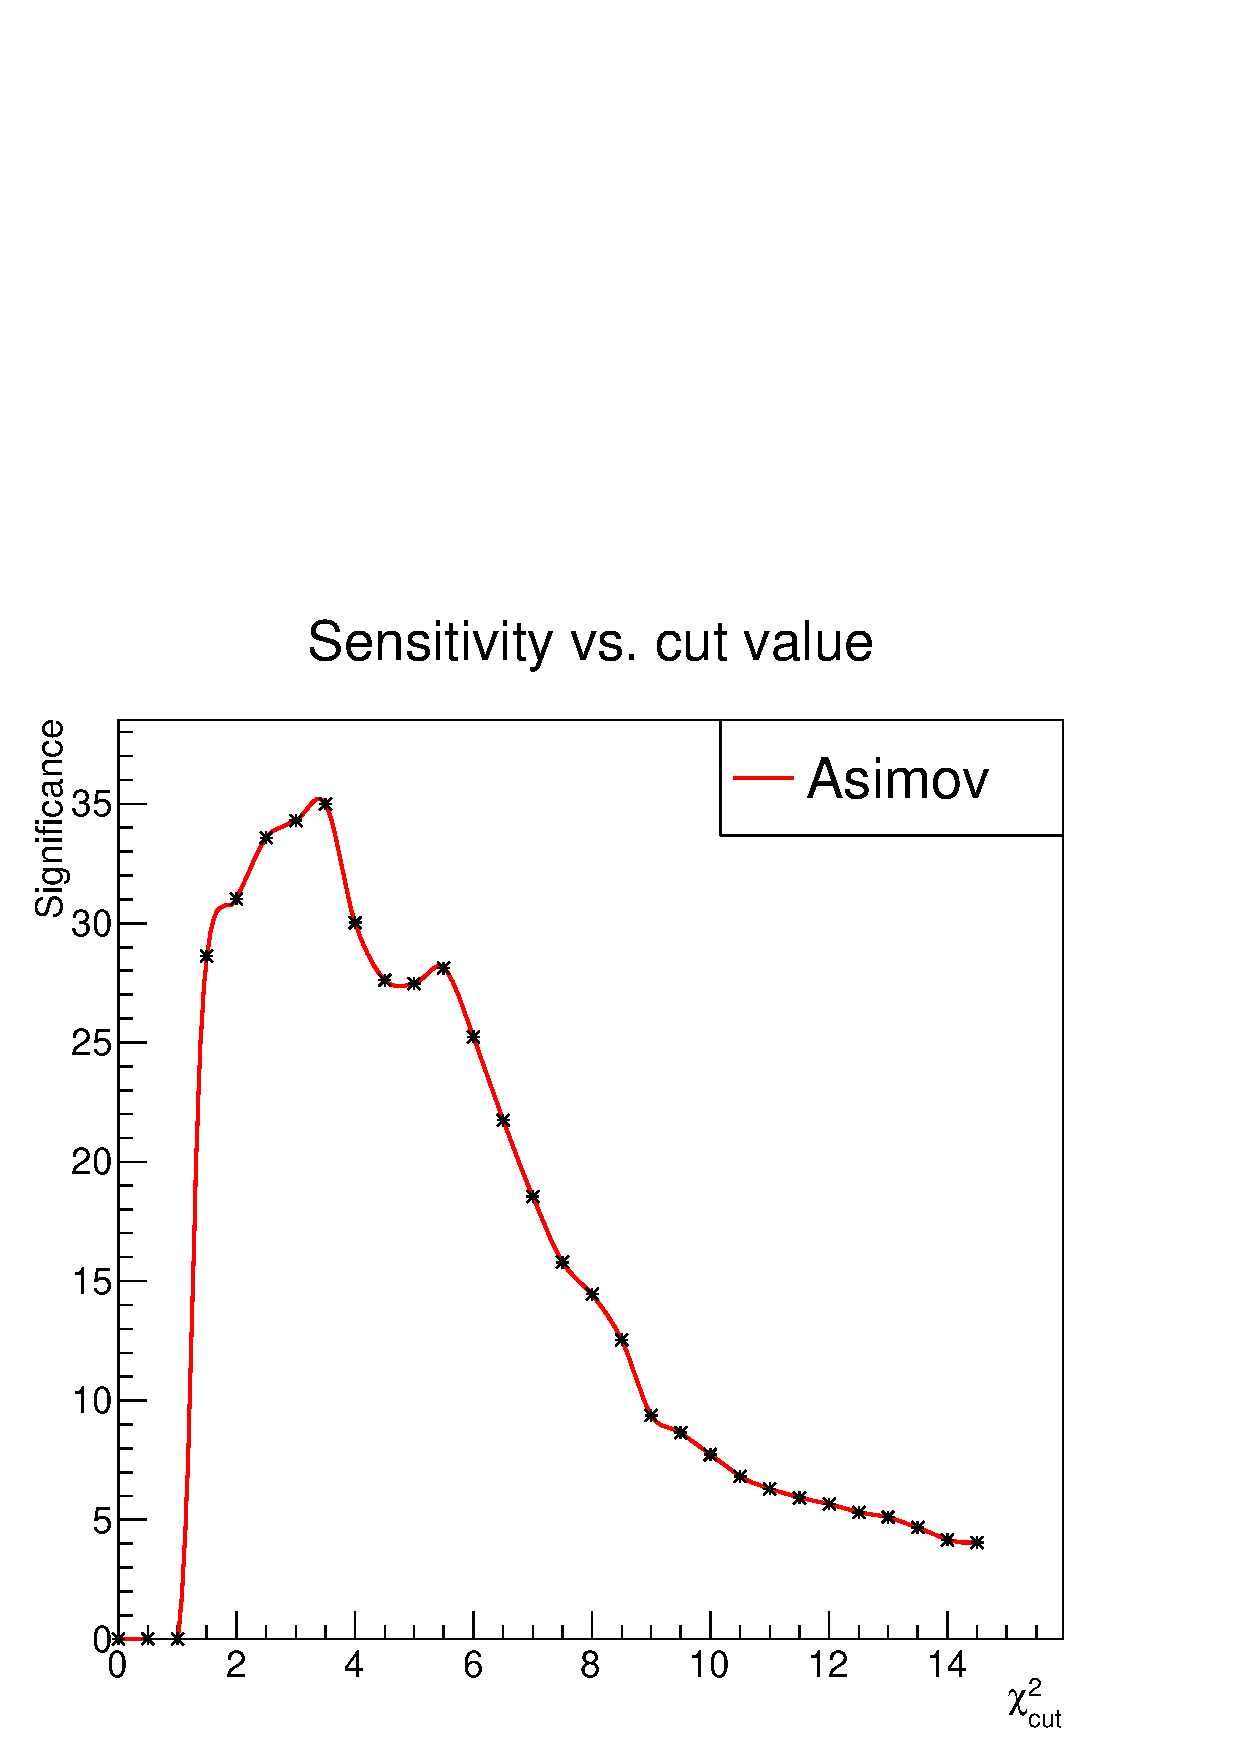
\includegraphics[scale=0.325]{img/sigcomp.pdf}
    \end{figure}\end{column}
    % \begin{column}{0.5\textwidth}\begin{figure}
    %   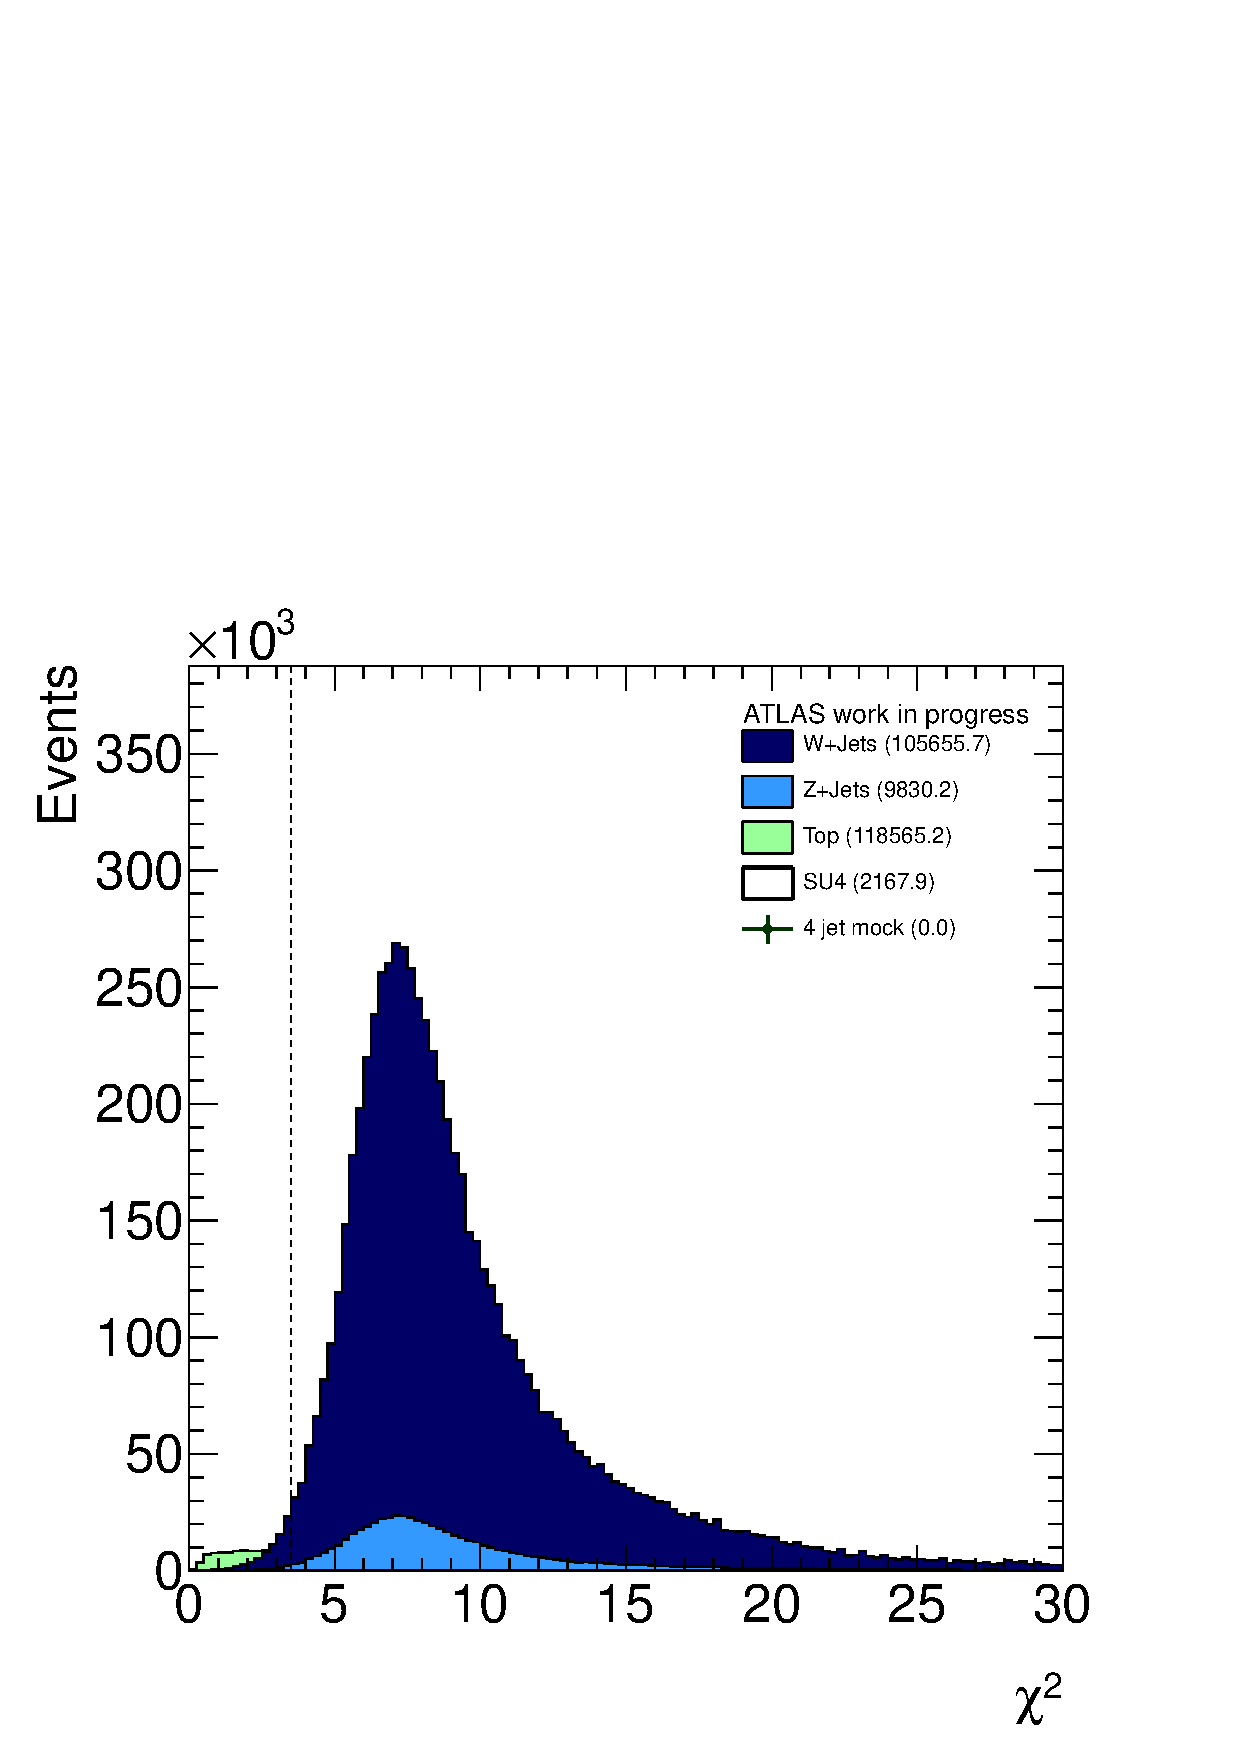
\includegraphics[scale=0.325]{img/Total__min_chi_all_all4.pdf}
    %   \caption{$\chi^2$ = $\chi^2_{kinematic} + \chi^2_{B}$}
    % \end{figure}\end{column}
  \end{columns}
\end{frame}

%\begin{frame}
%Using the $\chi^2$ as a descriminate alone gives $t\bar{t}$ purity $\approx80\%$ in $t\bar{t}$ samples where all decay products are reconstructed.
%
%Total $t\bar{t}$ purity including backgrounds is $\mathcal{O}\left(60\%\right)$.
%
%Further descrimination may be obtained by looking at likelihoods for the event maps.
%
%\end{frame}
%
%\begin{frame}
%We can form a probability of correct assignment, using the likelihood for a correct map;
%  \begin{equation}\begin{split}
%    L\left(a,b,c,d\right) =&
%    \frac{1}{\sqrt{2\pi}\sigma_{W_{h}}} \exp^{-\left(m_{ab}-M_{W}\right)^{2} / 2\sigma^{2}_{W_{h}}}
%    \frac{1}{\sqrt{2\pi}\sigma_{t_{h}}} \exp^{-\left(m_{abc}-m_{t}\right)^{2} / 2\sigma^{2}_{t_{h}}}
%    \\&\times
%    \frac{1}{\sqrt{2\pi}\sigma_{W_{l}}} \exp^{-\left(m_{dl\nu}-m_{t}\right)^{2} / 2\sigma^{2}_{t_{l}}}
%    \\&\times
%    L_{W}\left(\omega_{a},\omega_{b}\right) L_{bb}\left(\omega_{c},\omega_{d}\right),
%  \end{split}\end{equation}
%by summing all likelihoods where jets $a$ \& $b$ are assigned to the hadronic W.
%\begin{equation}
%P_{CA} = \frac{L\left(a,b,c,d\right) + L\left(a,b,d,c\right) + L\left(b,a,c,d\right) + L\left(b,a,d,c\right)}{\sum_{\text{all maps}} L\left(\text{map}\right)}
%\end{equation}
%\end{frame}

\section{Performance}

\begin{frame}{2 jet + Missing ET selection}
Test technique with loose SUSY selection:
\begin{itemize}
\item Require 2 tight leptons
\item Invariant mass of leptons $> 12\text{GeV}$
\item 2 jets, each with $p_T > 50\text{GeV}$
\item Missing $E_T > 220\text{GeV}$
\end{itemize}
Estimate yields at $25\text{fb}^{-1}$ (though still at $7 \text{TeV}$)
\end{frame}

\begin{frame}{2 jet + Missing ET selection}
  \begin{columns}
    \begin{column}{0.5\textwidth}\begin{figure}
      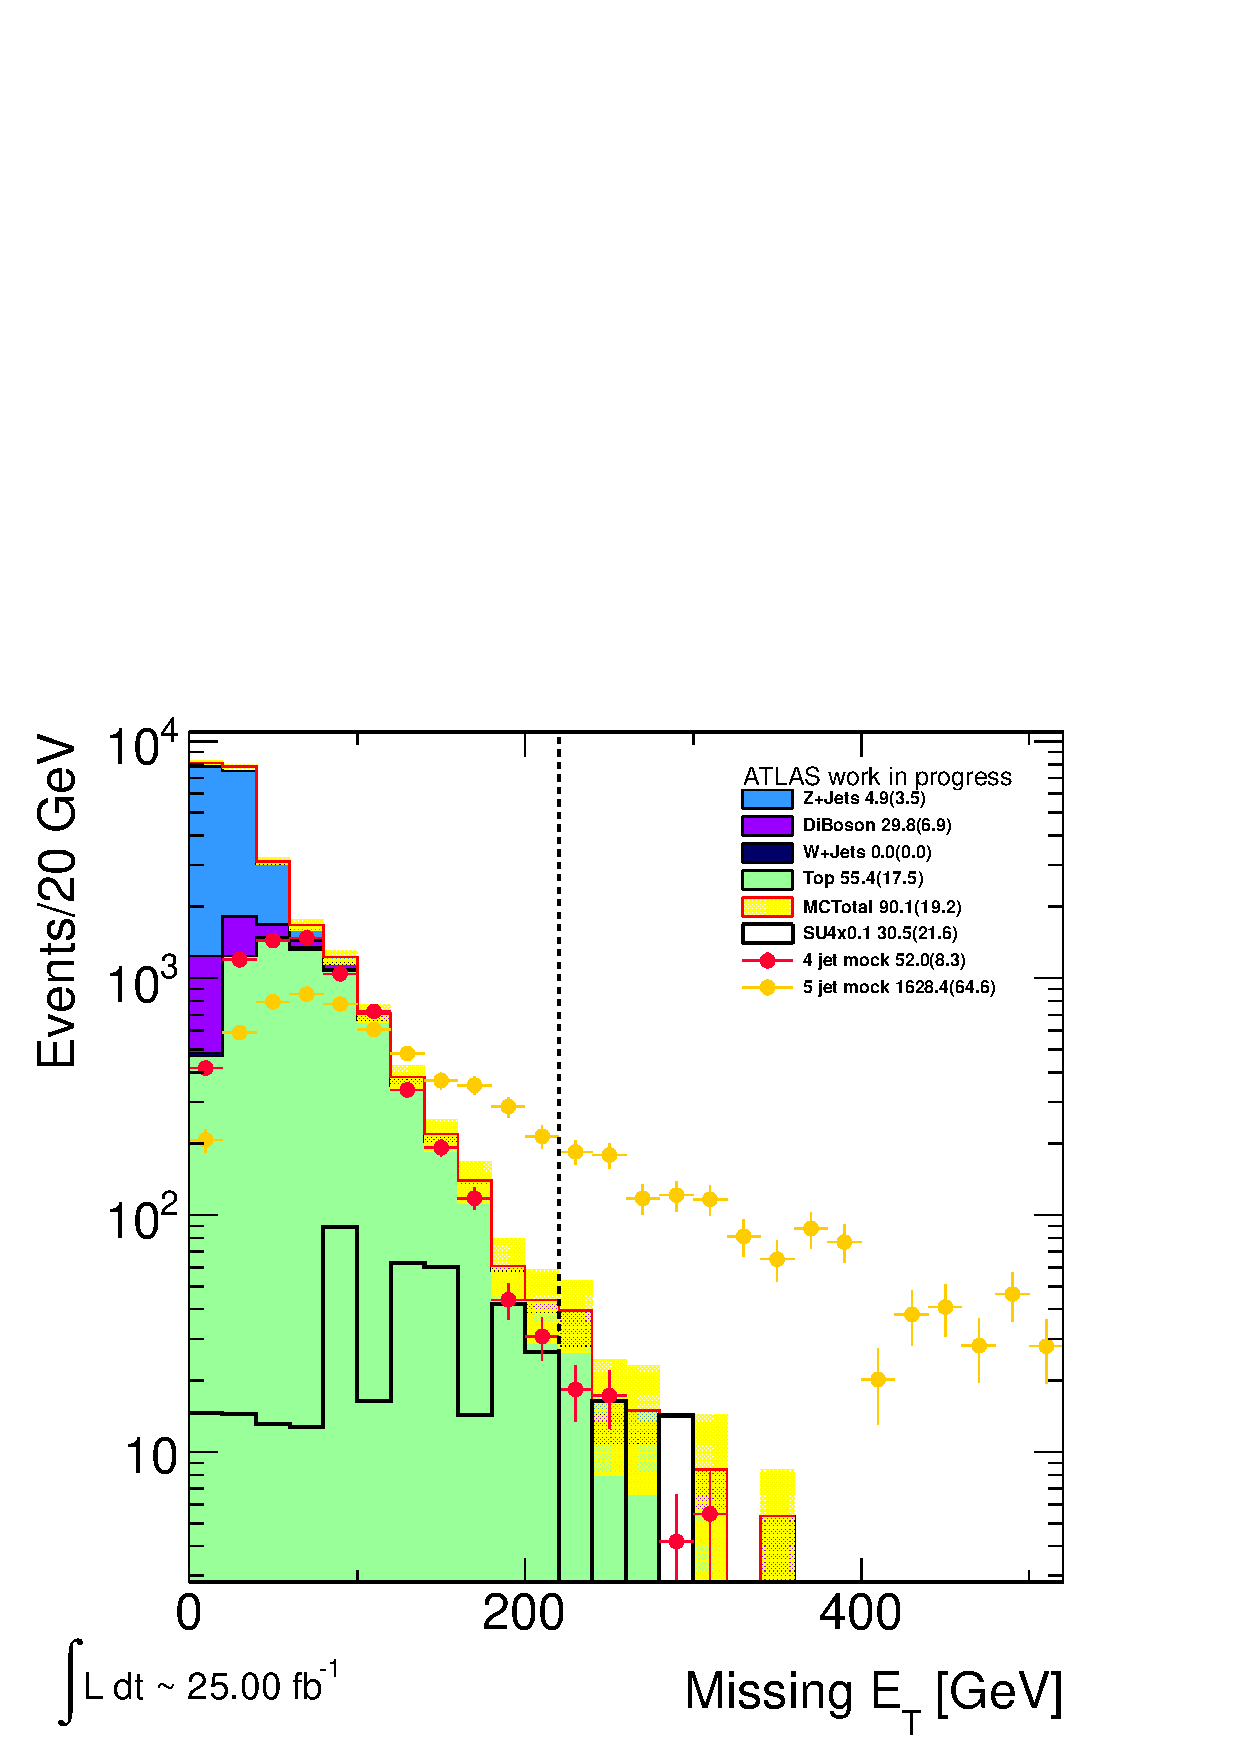
\includegraphics[scale=0.325]{img/Total_OS_EE_etmiss_2jet.pdf}
      \caption{$e^{+}e^{-}\slashed{E}_{T}$}
    \end{figure}\end{column}
    \begin{column}{0.5\textwidth}\begin{figure}
      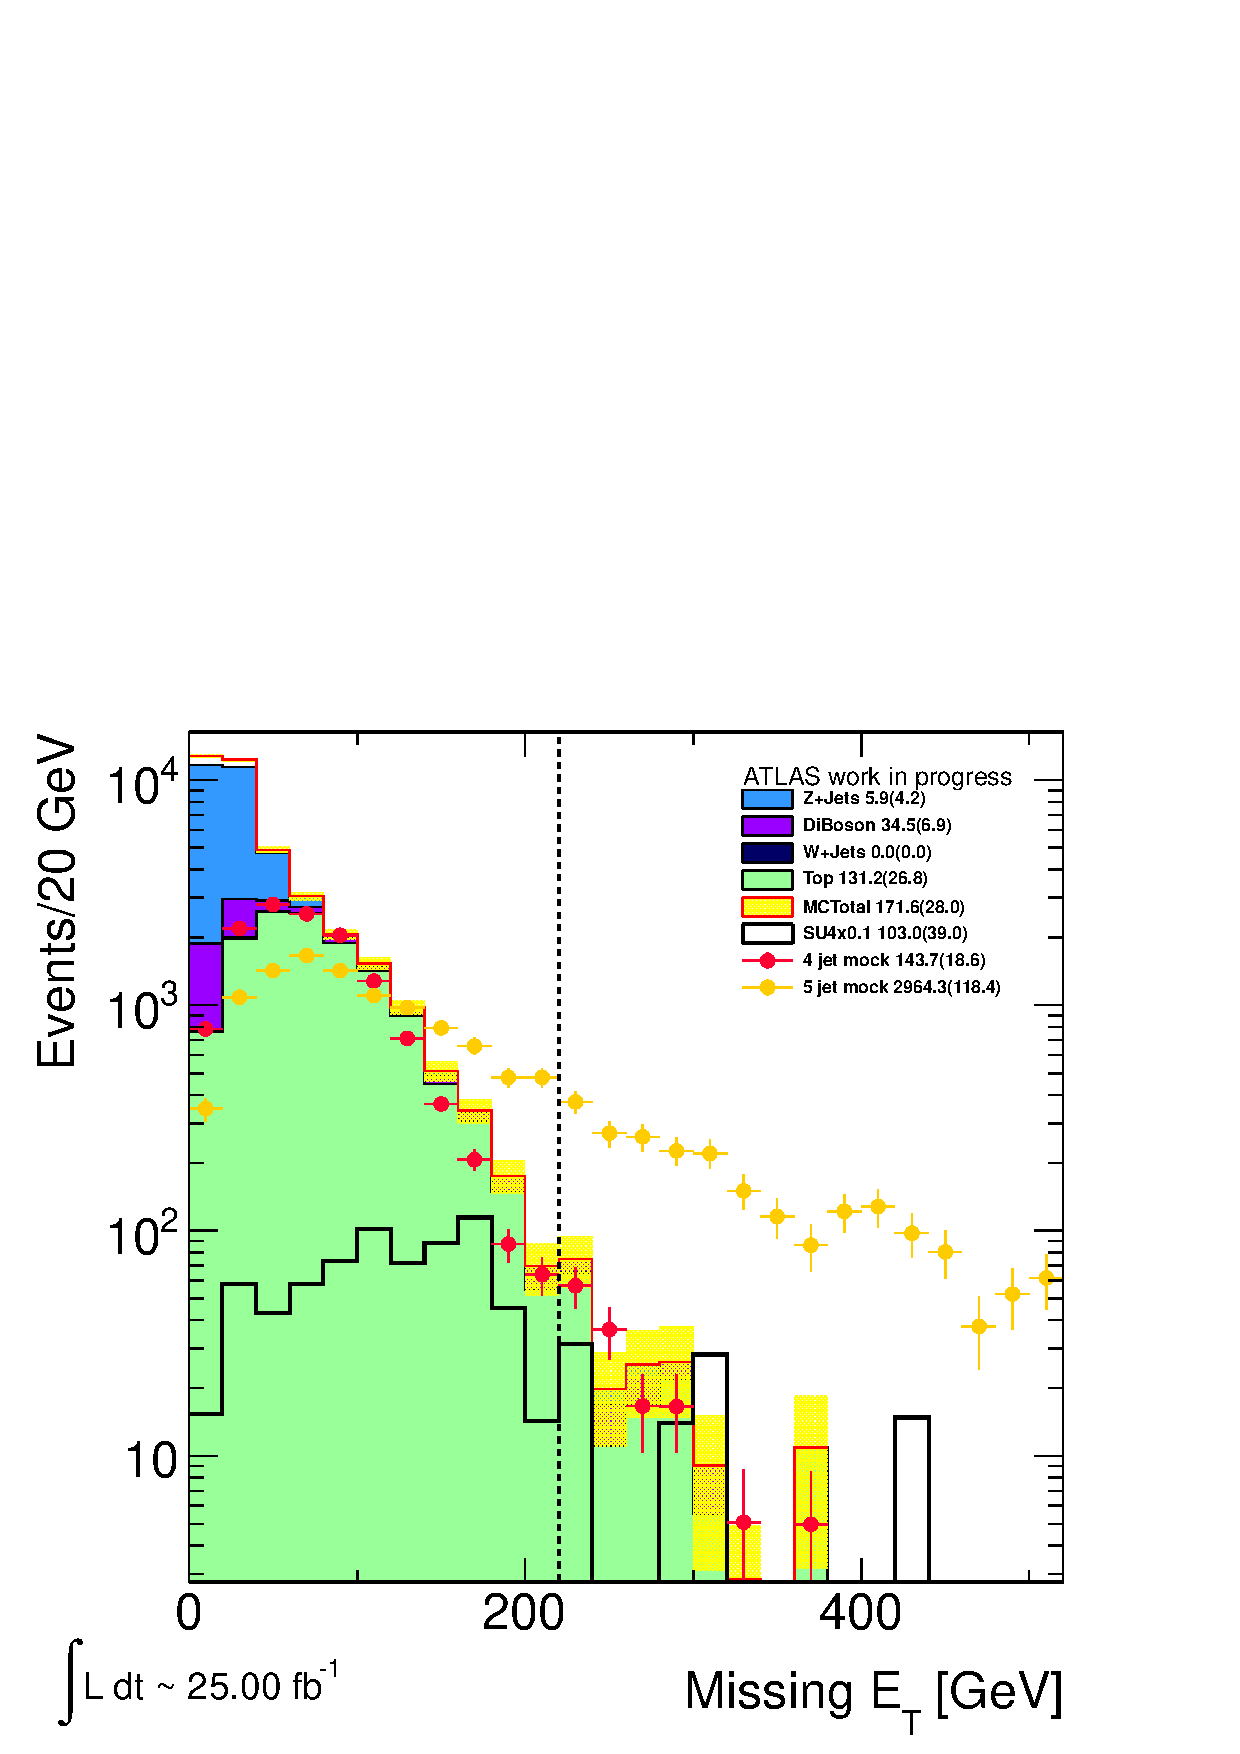
\includegraphics[scale=0.325]{img/Total_OS_MM_etmiss_2jet.pdf}
      \caption{$\mu^{+}\mu^{-}\slashed{E}_{T}$}
    \end{figure}\end{column}
  \end{columns}
\end{frame}

% \begin{frame}{2 jet + Missing ET selection}
%   \begin{columns}
%     \begin{column}{0.45\textwidth}\begin{figure}
%       \caption{$e^{\pm}\mu^{\mp}\slashed{E}_{T}$}
%       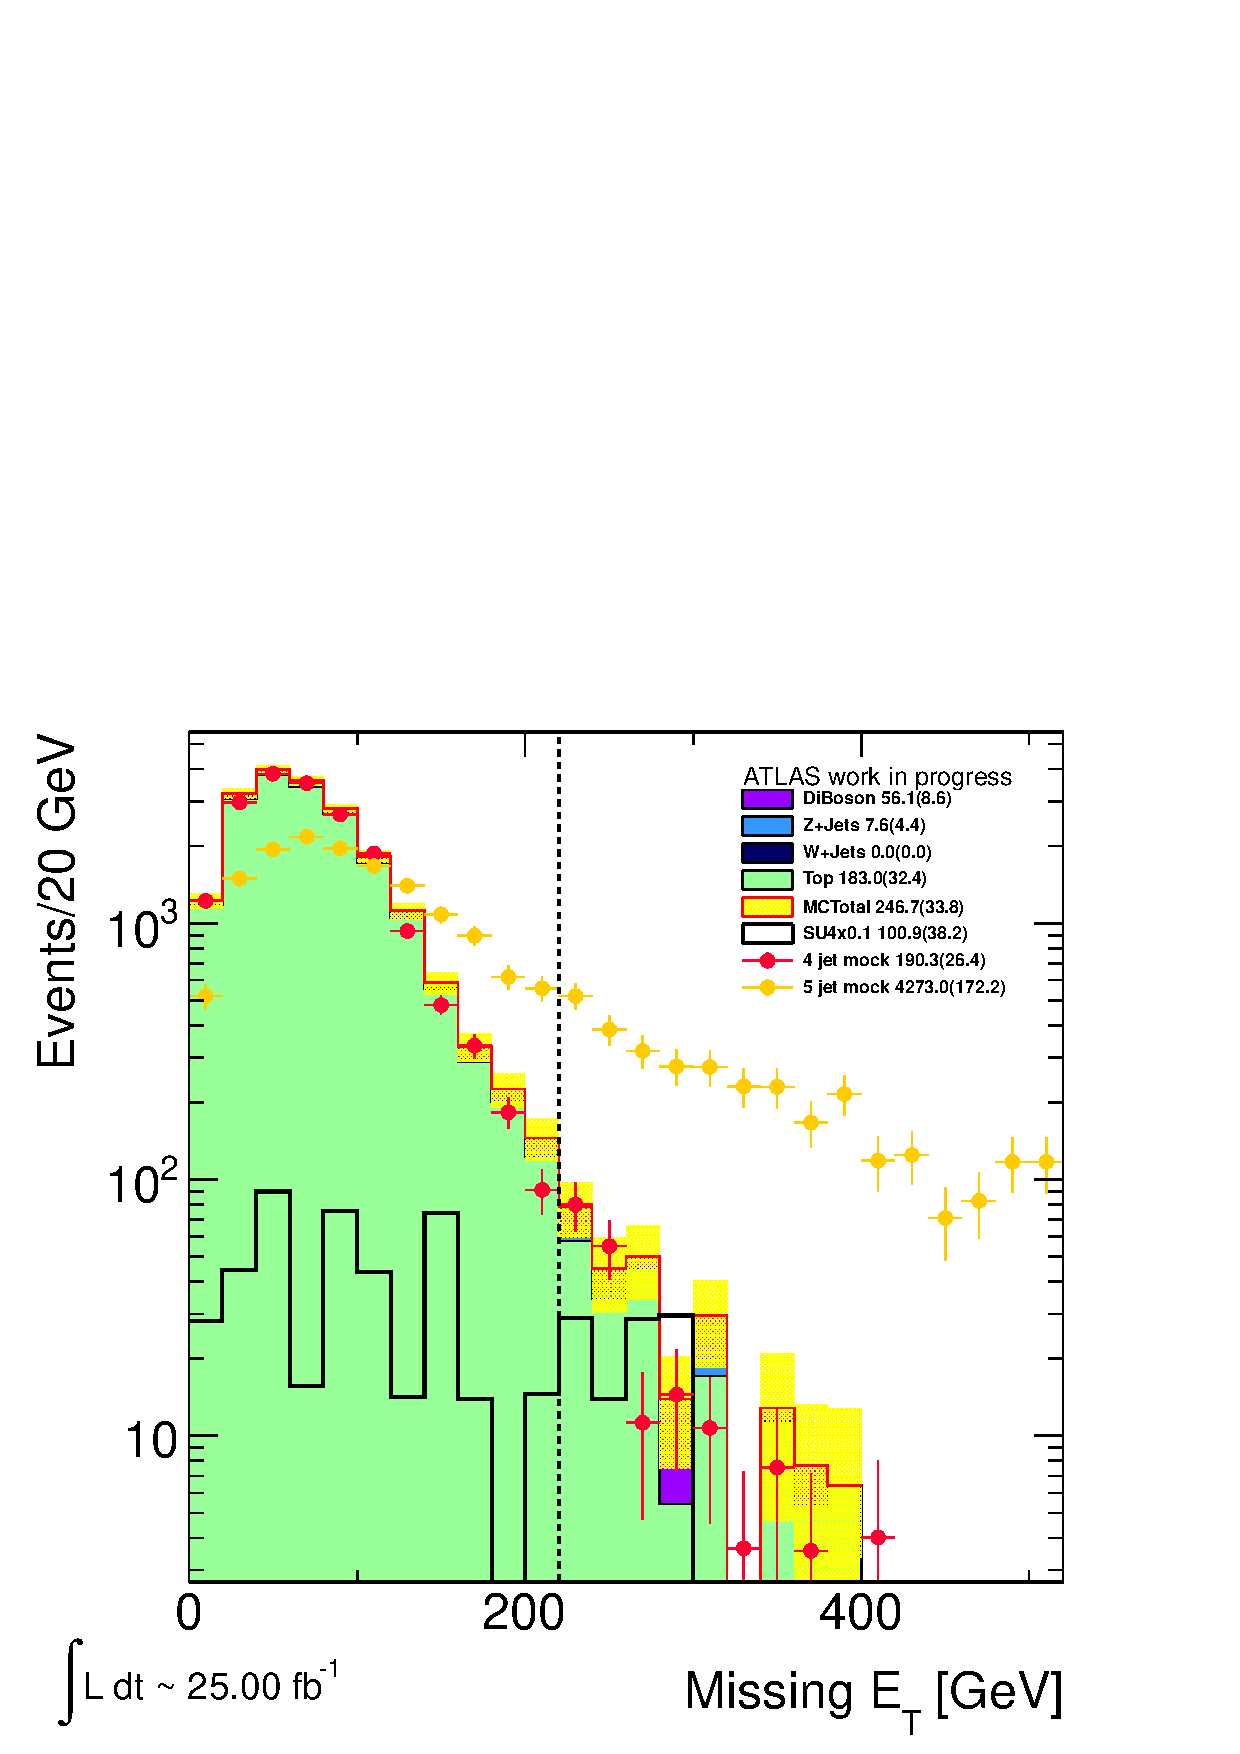
\includegraphics[scale=0.275]{img/Total_OS_EM_etmiss_2jet.pdf}
%     \end{figure}\end{column}
%     \begin{column}{0.45\textwidth}\begin{figure}
%       \caption{$\mu^{\pm}e^{\mp}\slashed{E}_{T}$}
%       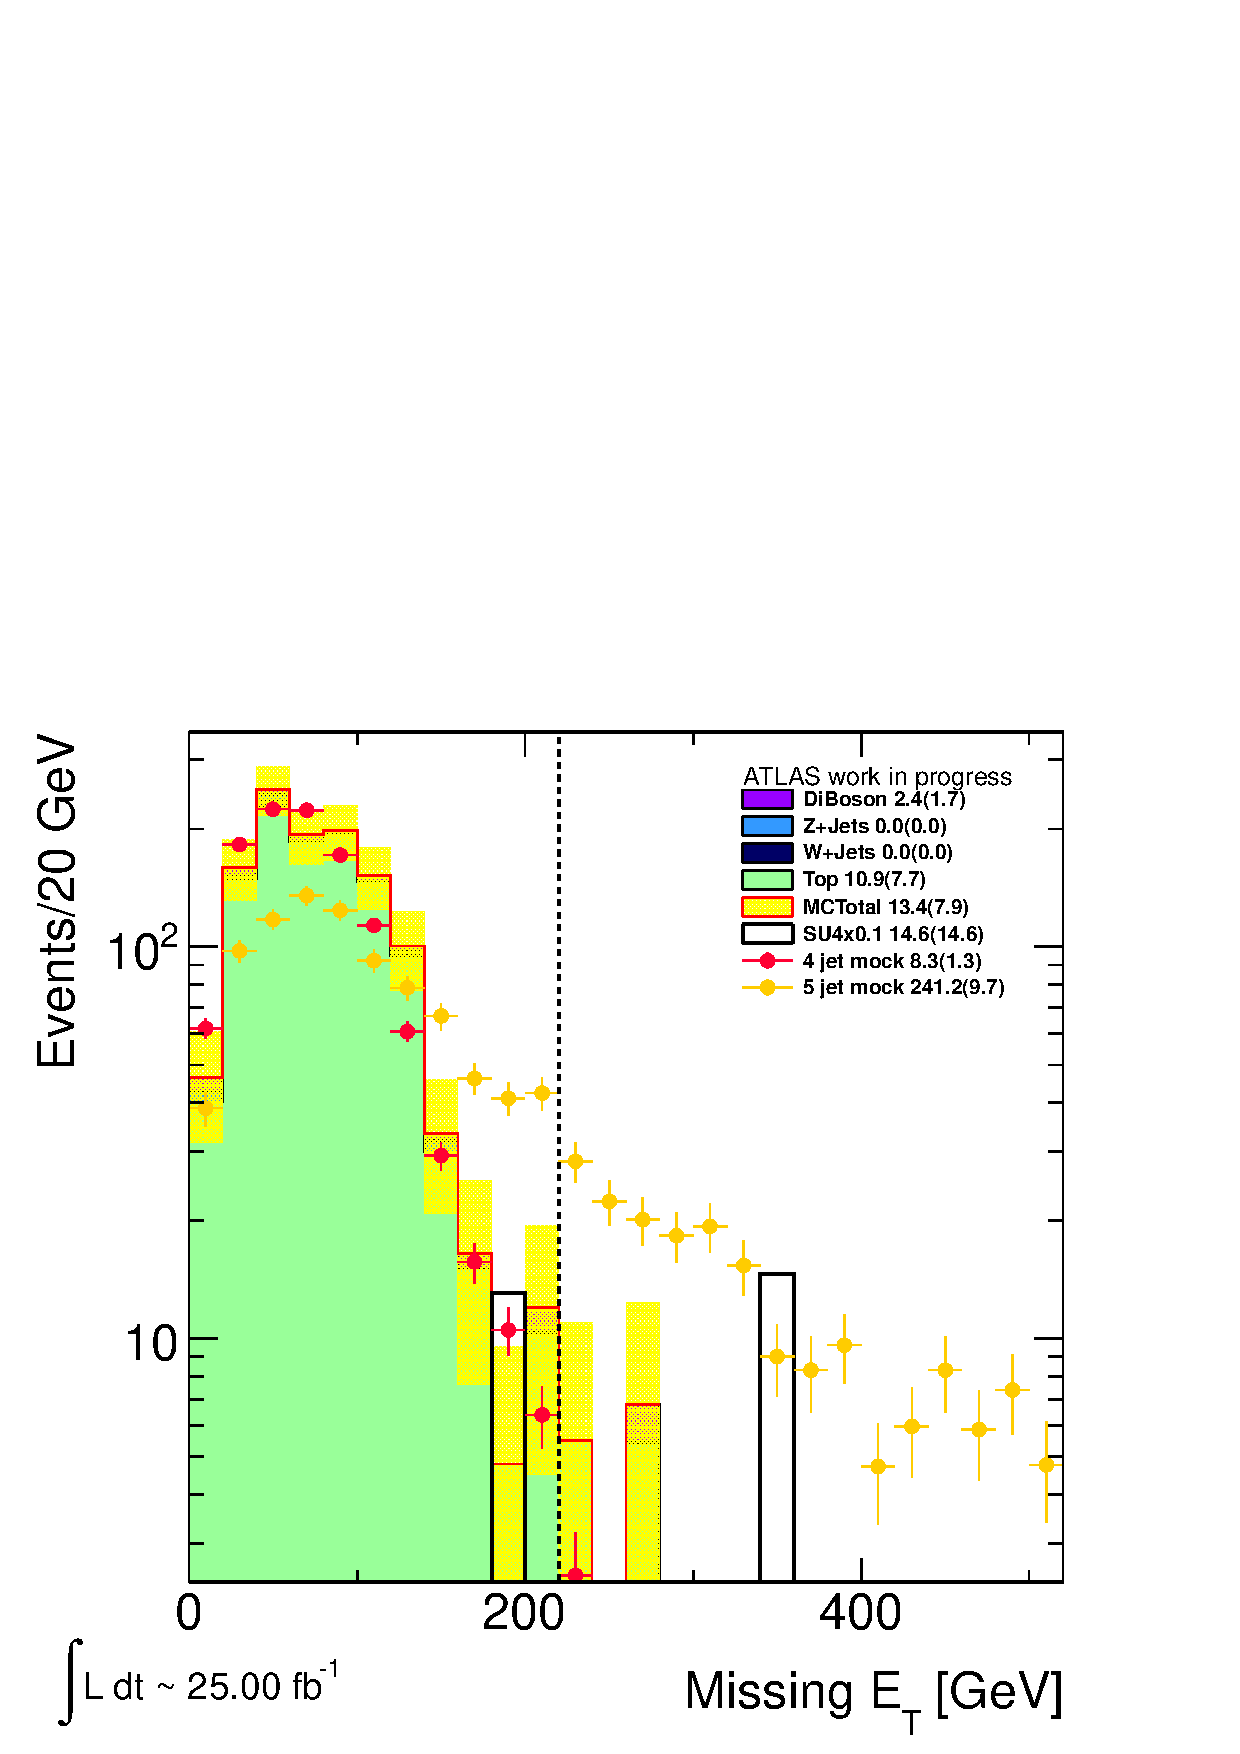
\includegraphics[scale=0.275]{img/Total_OS_ME_etmiss_2jet.pdf}
%     \end{figure}\end{column}
%   \end{columns}
% \end{frame}

% \begin{frame}{Estimates}
% \begin{table}
% \centering
% \begin{tabular}{c||r|r}
%                      & $e^+e^- $ & $\mu^+\mu^-$ \\
% \hline \hline
% W+Jets    & $0.0$         & $0.0$ \\
% Z+Jets    & $4.9\pm3.5$   & $5.9\pm4.2$ \\
% DiBoson   & $29.8\pm6.9$  & $34.5\pm$ \\
% MC Top    & $55.4\pm17.5$ & $131.2\pm$ \\
% 4jet mock & $52.0\pm8.3$  & $143.7\pm18.6$ \\
% \hline
% MC Total  & $90.1\pm19.2$ & $171.6\pm28.0$ \\
% Mock Total& $86.7\pm11.4$ & $184.0\pm20.2$ \\
% \hline
% SU4x0.1   & $30.5\pm21.6$ & $103.0\pm39.0$ \\
% \hline
% \end{tabular}
% %\caption{This table shows some data}
% \label{tab:myfirsttable}
% \end{table}
% \end{frame}

% \begin{frame}{MC12 - Data12\_8TeV update}
% \begin{itemize}
%     \item Pileup weighting tool not working with data12 distributions
%     \item $\slashed{E}_{T}$ source changed and $sin(\Delta\phi)$ dependance added
%     \item Lowest unprescaled single electron Trigger now EF\_24vhi\_medium1
% \end{itemize}
% \end{frame}

% \begin{frame}{Further work}
%   \begin{itemize}
%     \item Finish update to latest release/prescriptions for $8\text{TeV}$ analysis.
%     \item Test procedure over range of SUSY models
%   \end{itemize}
% \end{frame}

%\begin{frame}{Thanks}
%  MC event graphs rendered with MCViz (\url{MCViz.net}).
%\end{frame}

% \begin{frame}{Jet pT}
%   \begin{columns}
%     \begin{column}{0.5\textwidth}\begin{figure}
%       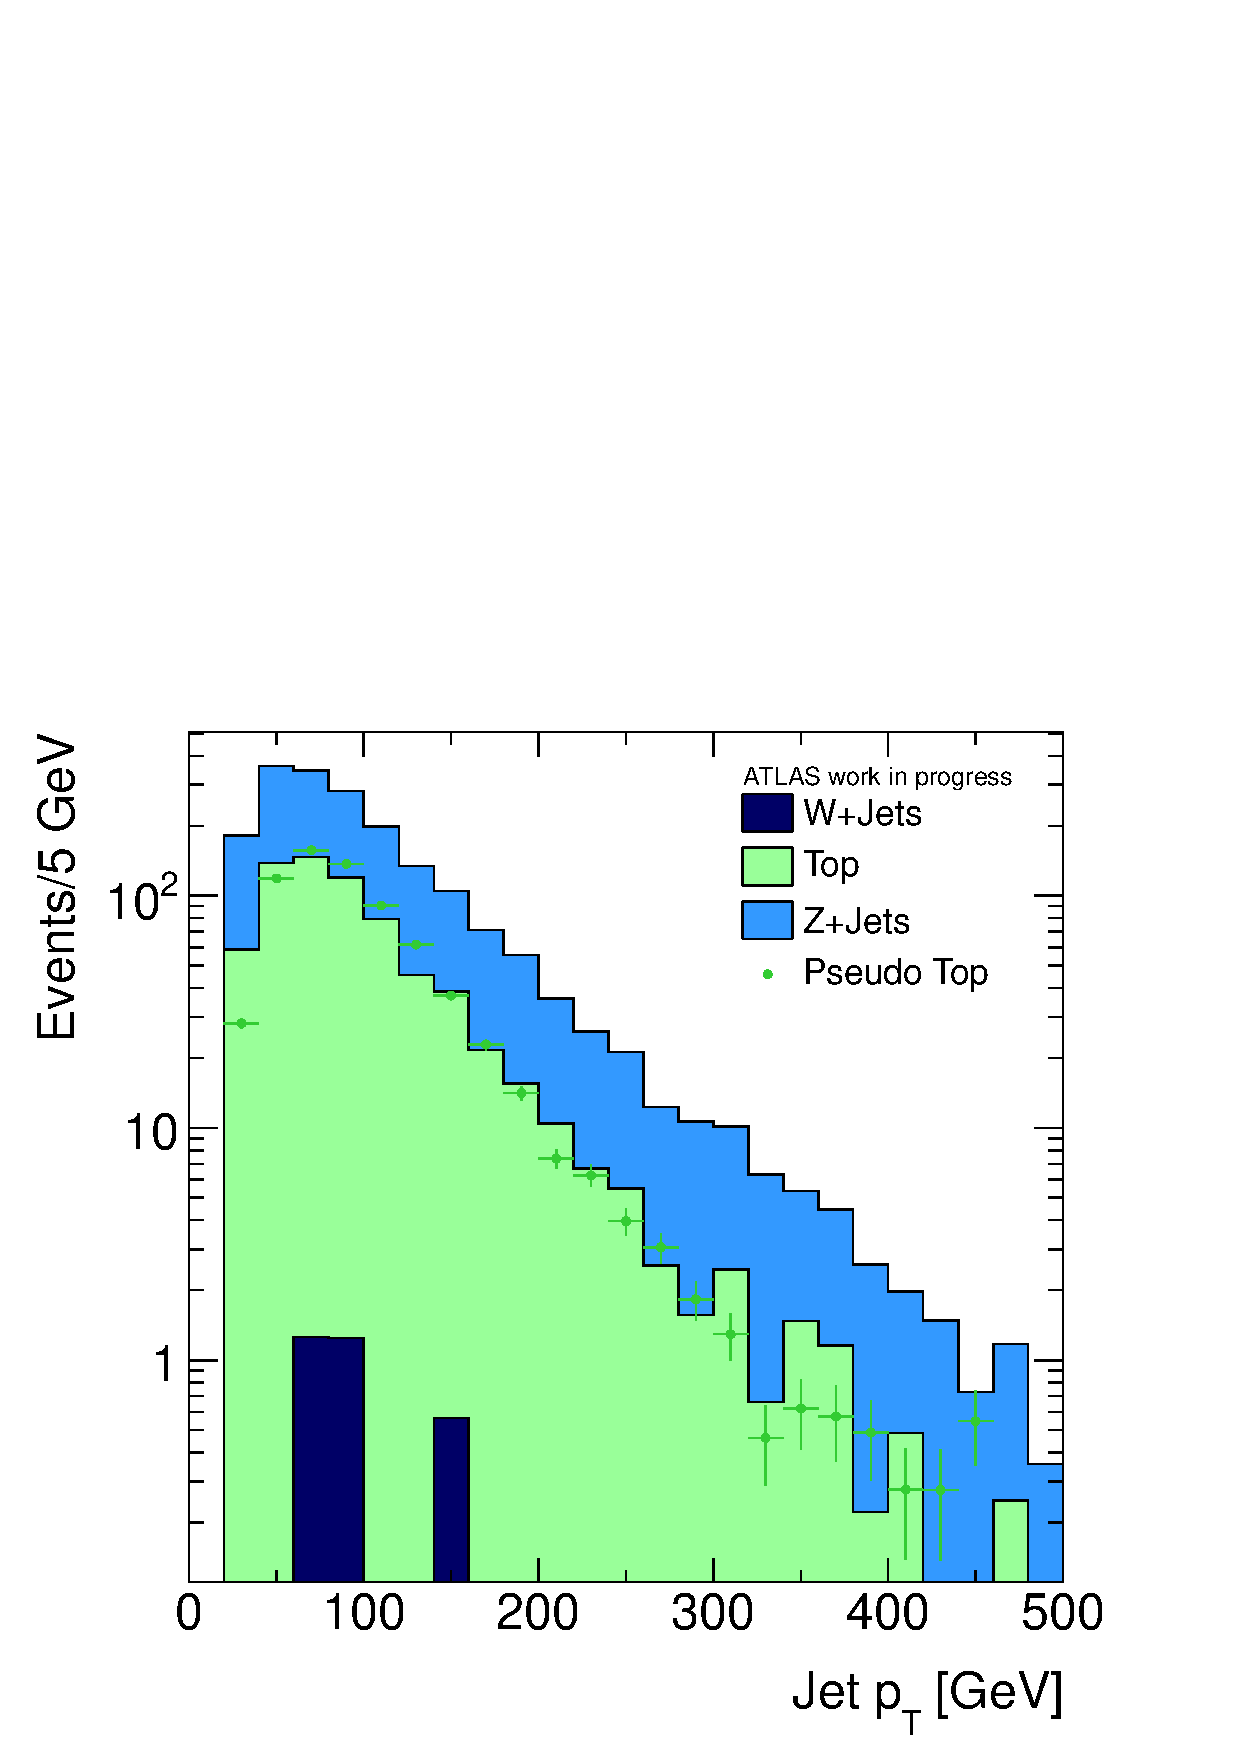
\includegraphics[scale=0.325]{img/Total_OS_EE_jet_lead_pt_scaled.pdf}
%       \caption{$e^{+}e^{-}p_{T}^{\text{jet 1}}$}
%     \end{figure}\end{column}
%     \begin{column}{0.5\textwidth}\begin{figure}
%       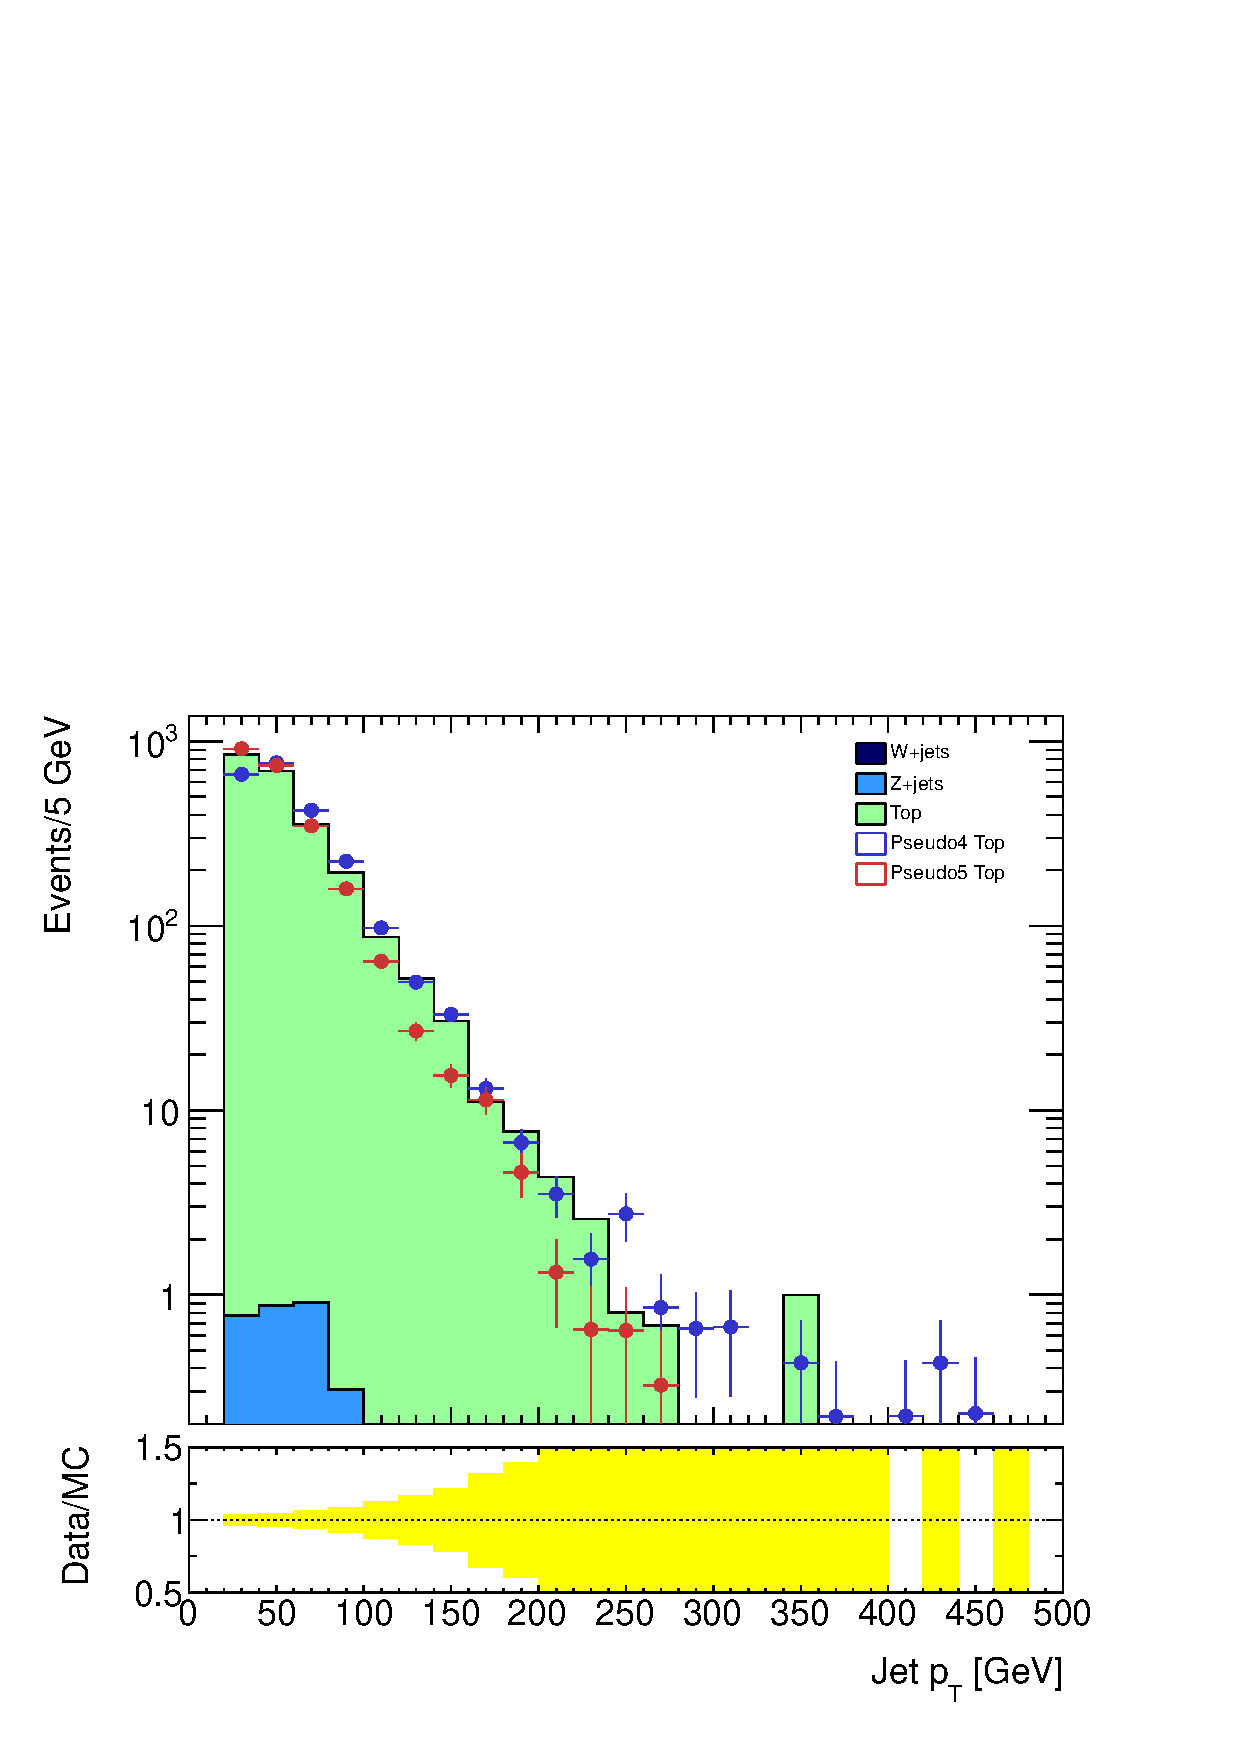
\includegraphics[scale=0.325]{img/Total_OS_EE_jet_lead2_pt_scaled.pdf}
%       \caption{$e^{+}e^{-}p_{T}^{\text{jet 2}}$}
%     \end{figure}\end{column}
%   \end{columns}
% \end{frame}

% \begin{frame}{Effective mass}
%   \begin{columns}
%     \begin{column}{0.5\textwidth}\begin{figure}
%       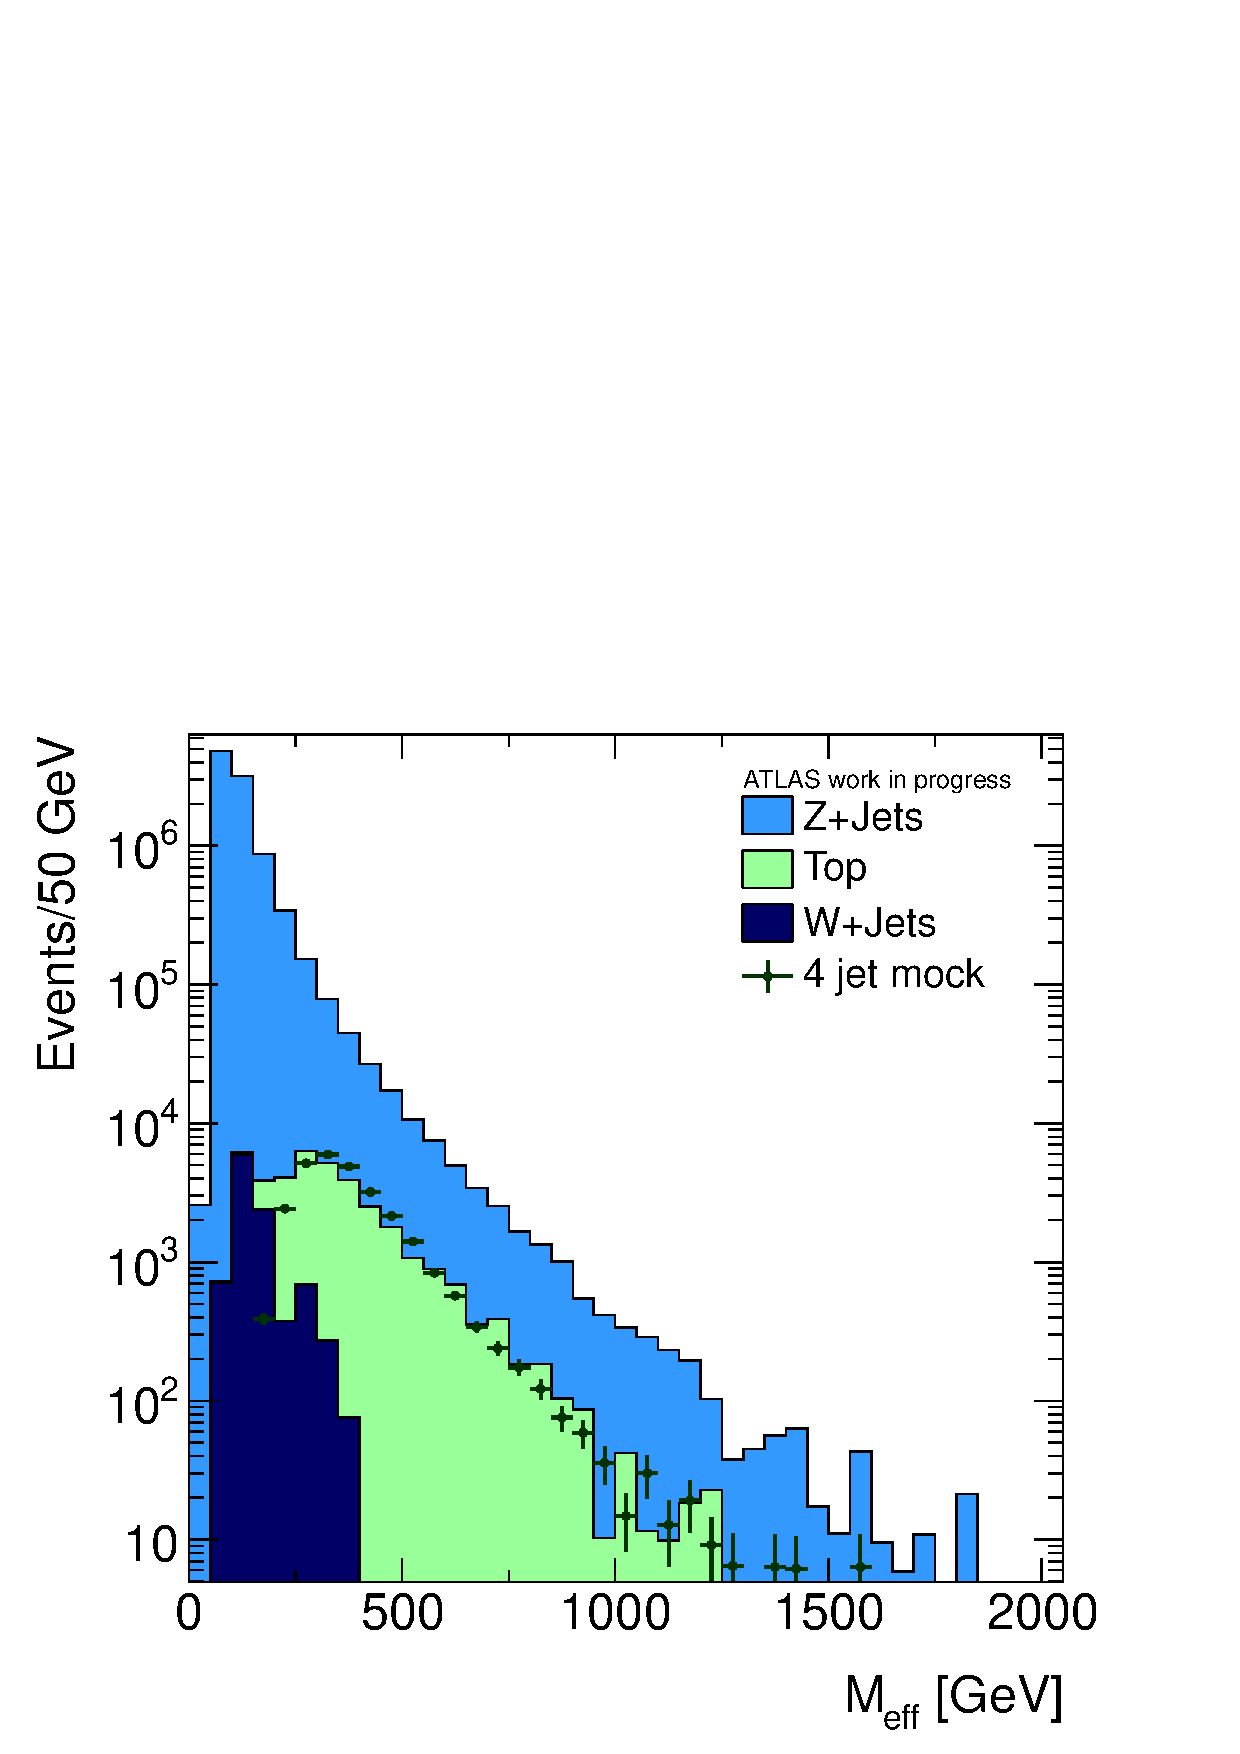
\includegraphics[scale=0.325]{img/Total_OS_EE_meff_scaled.pdf}
%       \caption{$e^{+}e^{-}\slashed{E}_{T}$}
%     \end{figure}\end{column}
%     \begin{column}{0.5\textwidth}\begin{figure}
%       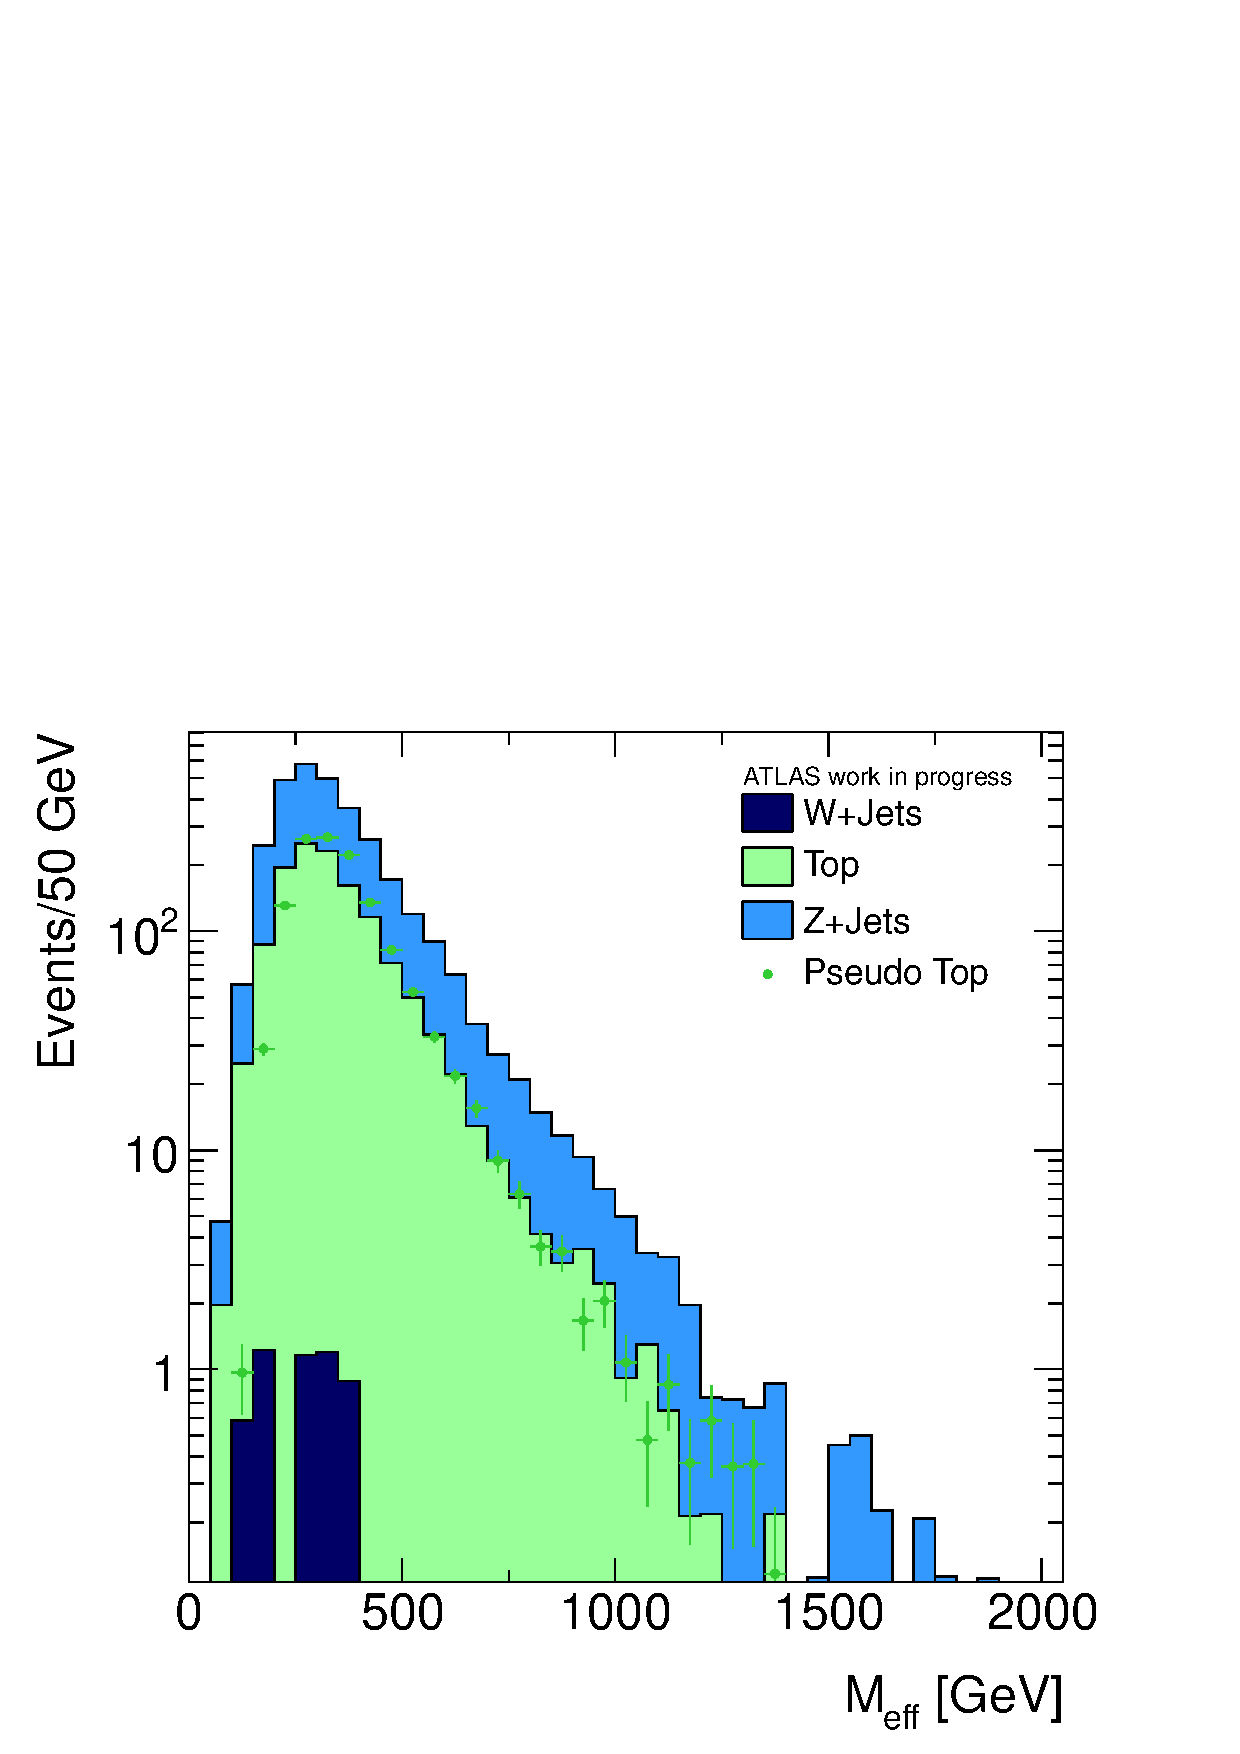
\includegraphics[scale=0.325]{img/Total_OS_MM_meff_scaled.pdf}
%       \caption{$\mu^{+}\mu^{-}\slashed{E}_{T}$}
%     \end{figure}\end{column}
%   \end{columns}
% \end{frame}

% \begin{frame}{Missing ET}
%   \begin{columns}
%     \begin{column}{0.5\textwidth}\begin{figure}
%       \caption{$e^{+}e^{-}\slashed{E}_{T}$}
%       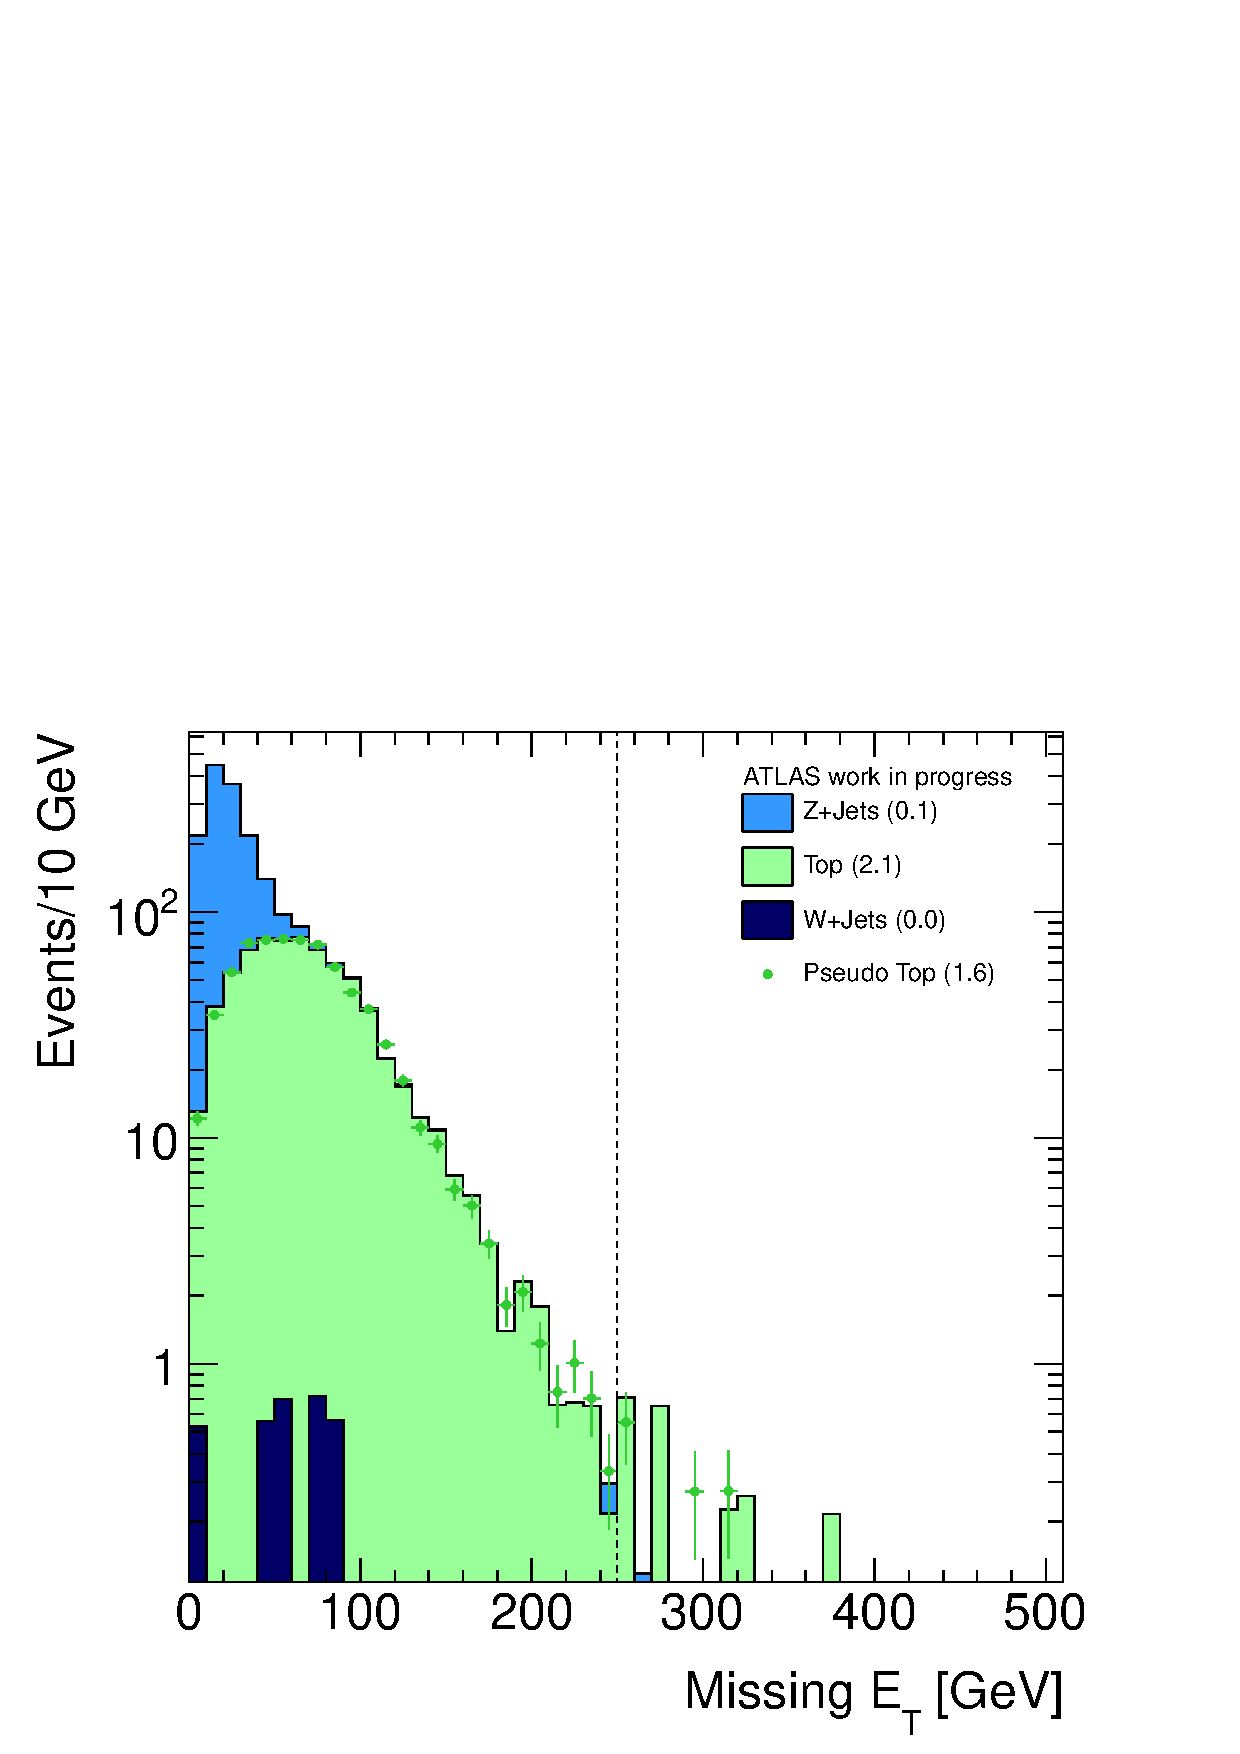
\includegraphics[scale=0.325]{img/Total_OS_EE_etmiss_scaled.pdf}
%     \end{figure}\end{column}
%     \begin{column}{0.5\textwidth}\begin{figure}
%       \caption{$\mu^{+}\mu^{-}\slashed{E}_{T}$}
%       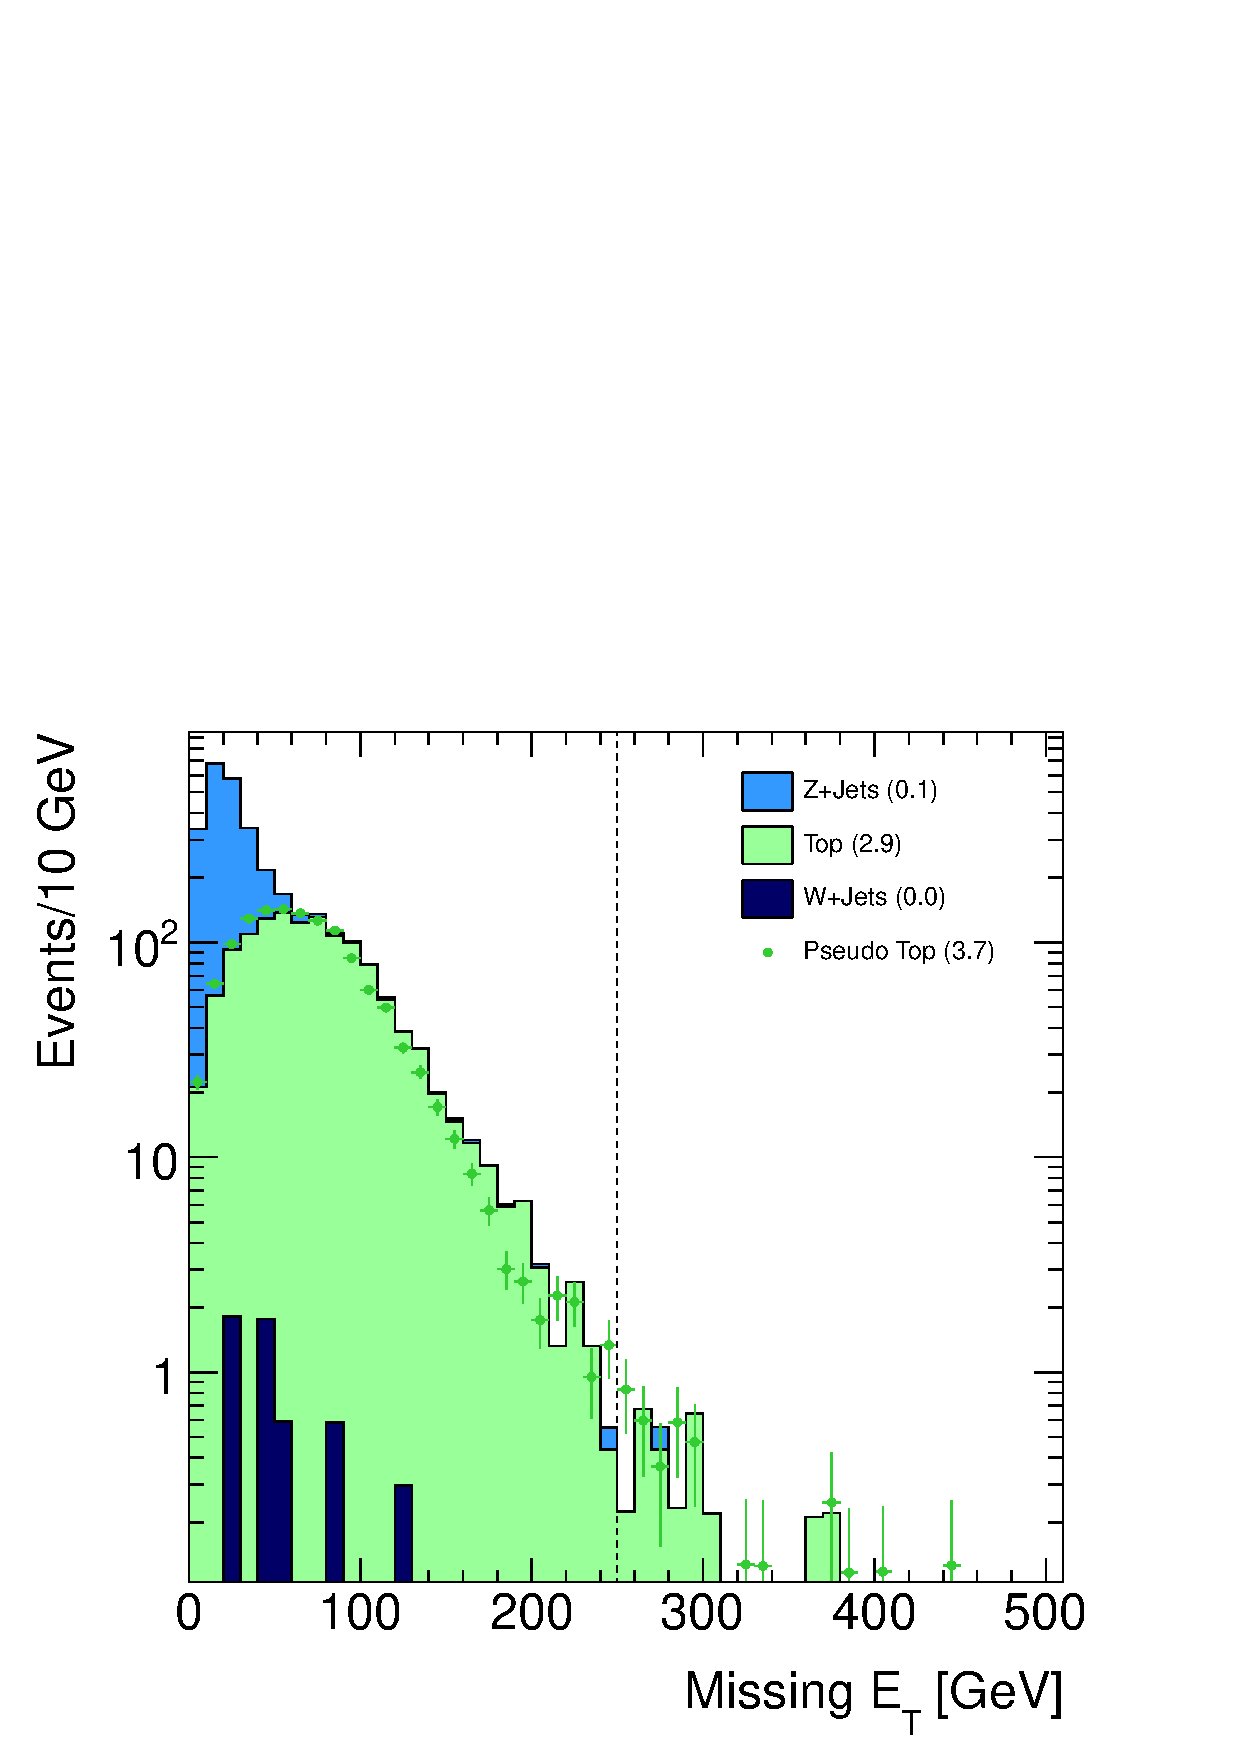
\includegraphics[scale=0.325]{img/Total_OS_MM_etmiss_scaled.pdf}
%     \end{figure}\end{column}
%   \end{columns}
% \end{frame}

% \begin{frame}{Effective mass - different flavour}
%   \begin{columns}
%     \begin{column}{0.5\textwidth}\begin{figure}
%       \caption{$e^{\pm}\mu^{\mp}\slashed{E}_{T}$}
%       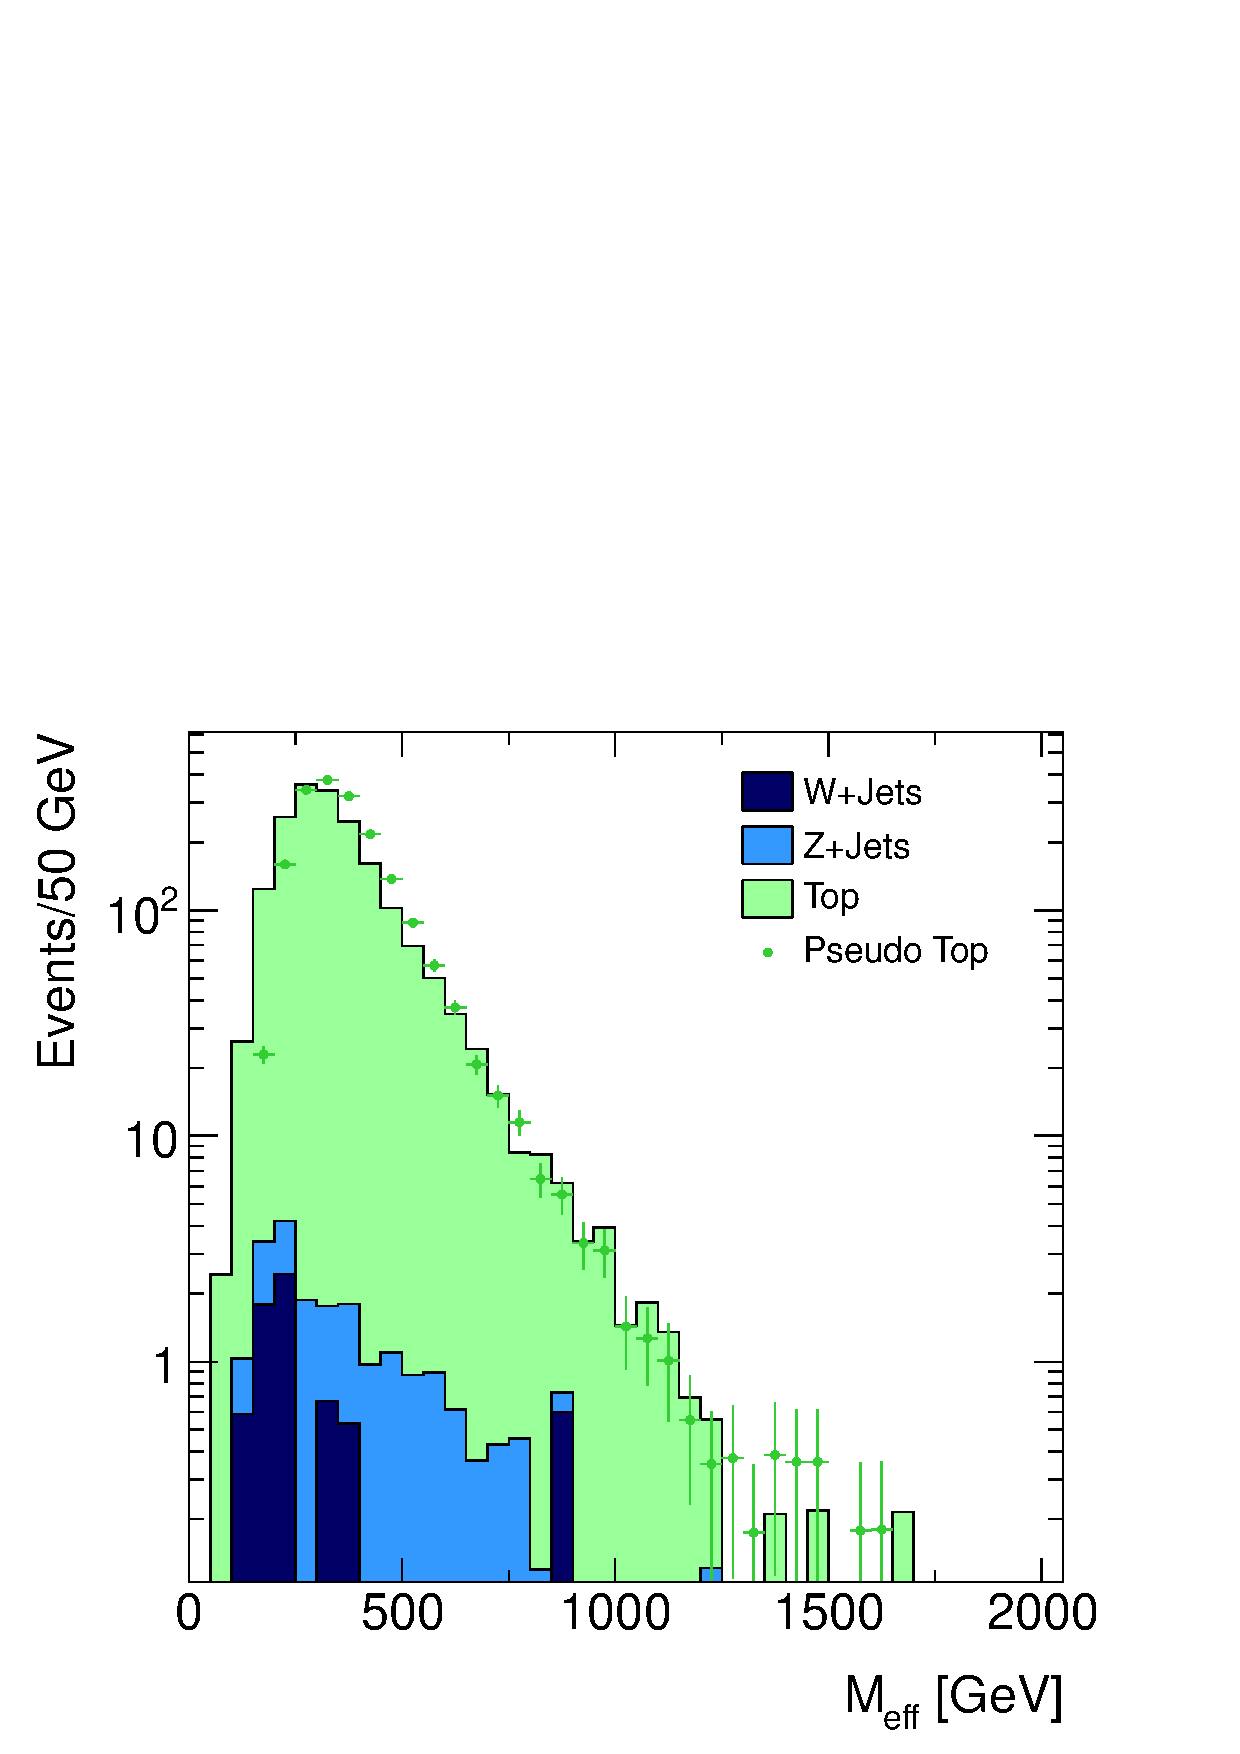
\includegraphics[scale=0.325]{img/Total_OS_EM_meff_scaled.pdf}
%     \end{figure}\end{column}
%     \begin{column}{0.5\textwidth}\begin{figure}
%       \caption{$\mu^{\pm}e^{\mp}\slashed{E}_{T}$}
%       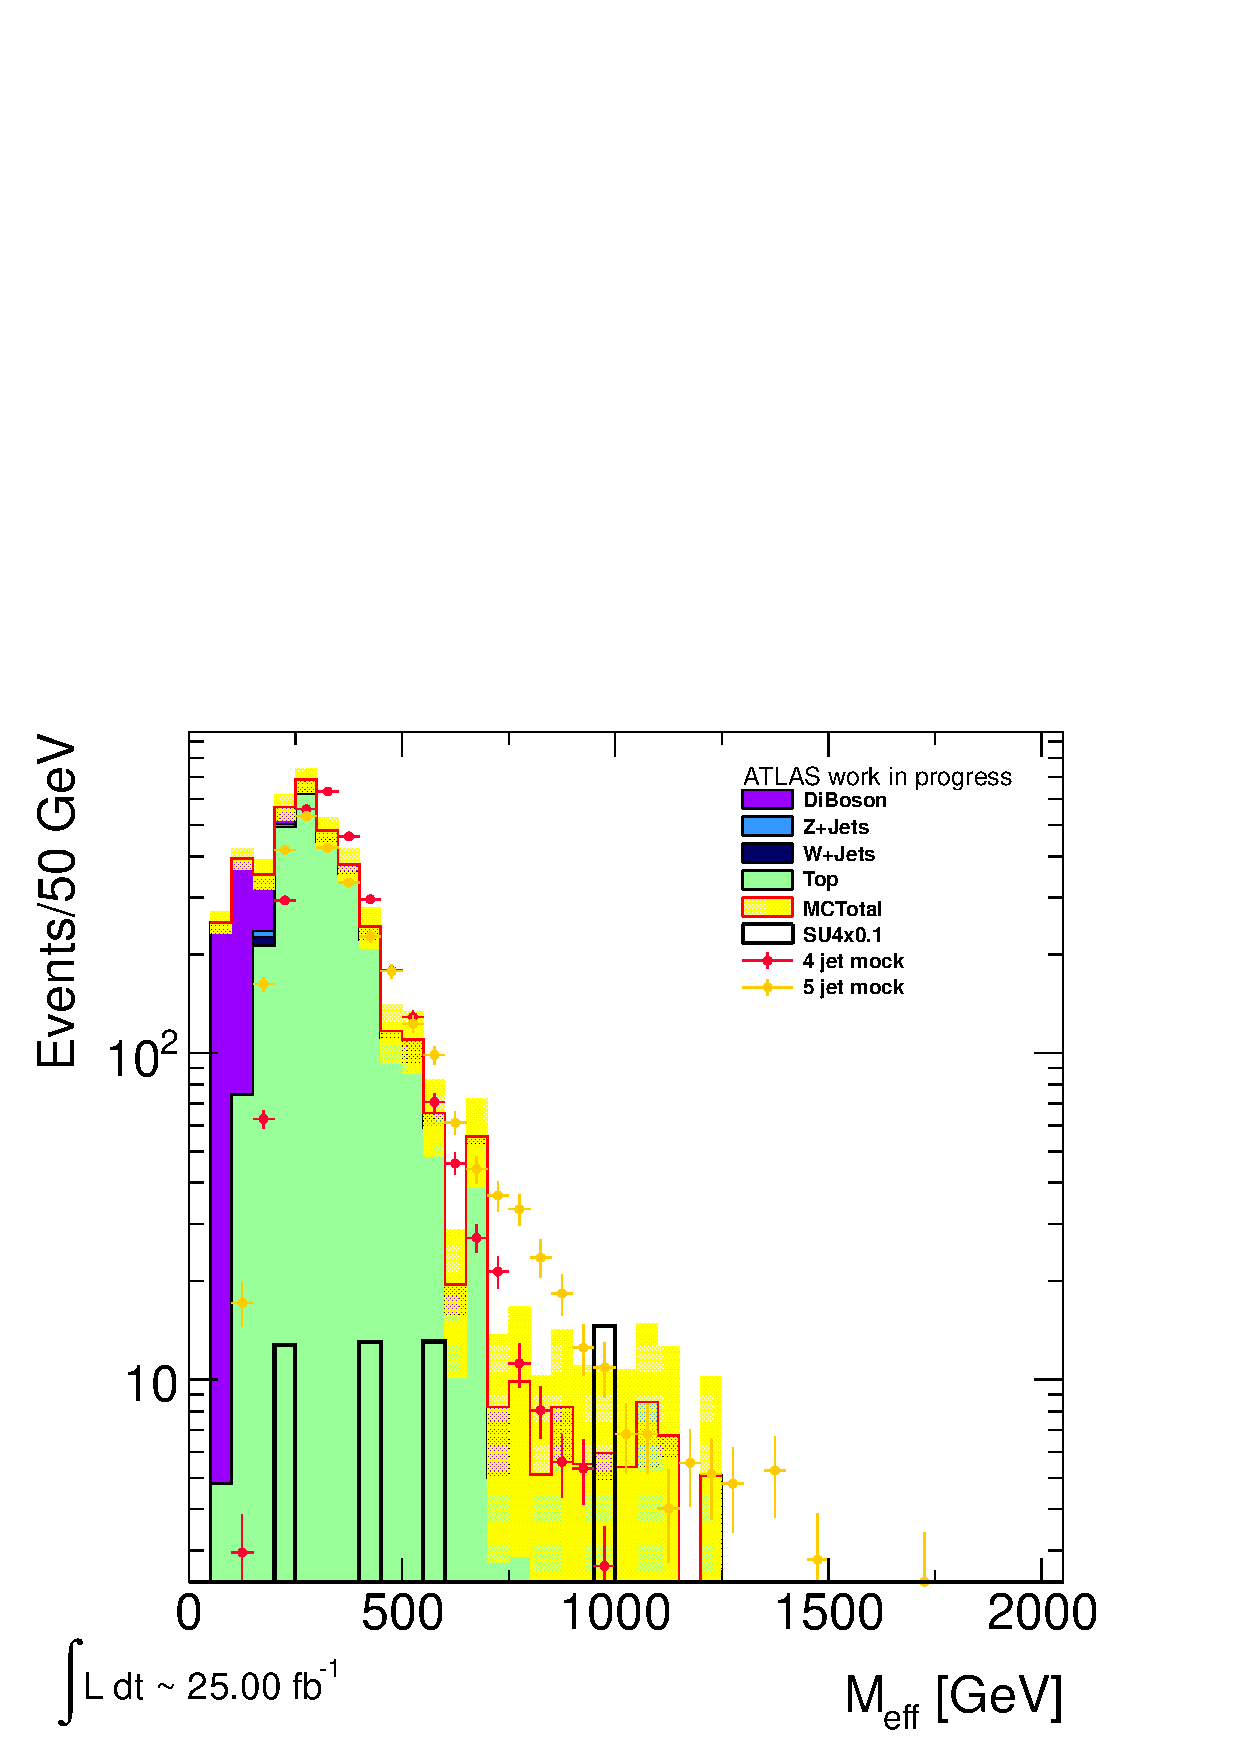
\includegraphics[scale=0.325]{img/Total_OS_ME_meff_scaled.pdf}
%     \end{figure}\end{column}
%   \end{columns}
% \end{frame}

% \begin{frame}{Missing ET - different flavour}
%   \begin{columns}
%     \begin{column}{0.5\textwidth}\begin{figure}
%       \caption{$e^{\pm}\mu^{\mp}\slashed{E}_{T}$}
%       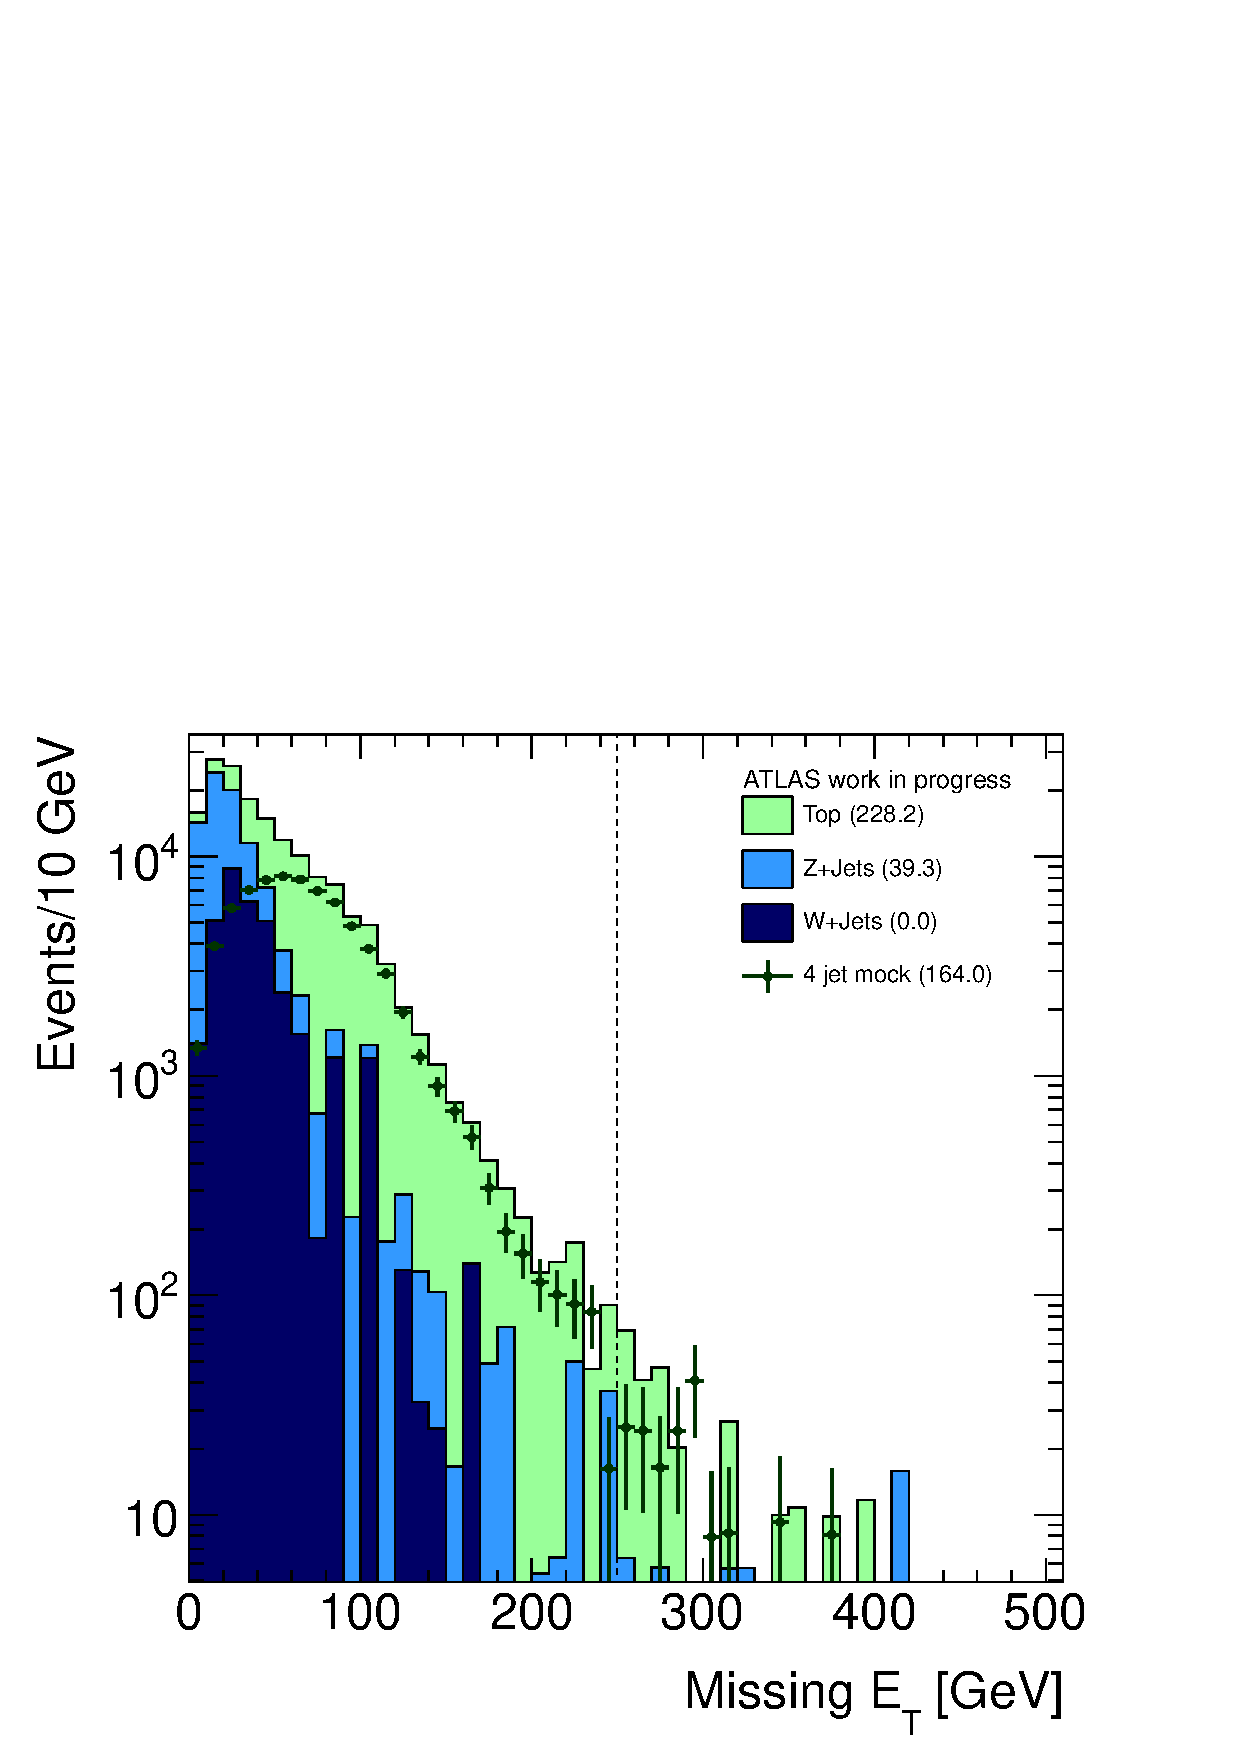
\includegraphics[scale=0.325]{img/Total_OS_EM_etmiss_scaled.pdf}
%     \end{figure}\end{column}
%     \begin{column}{0.5\textwidth}\begin{figure}
%       \caption{$\mu^{\pm}e^{\mp}\slashed{E}_{T}$}
%       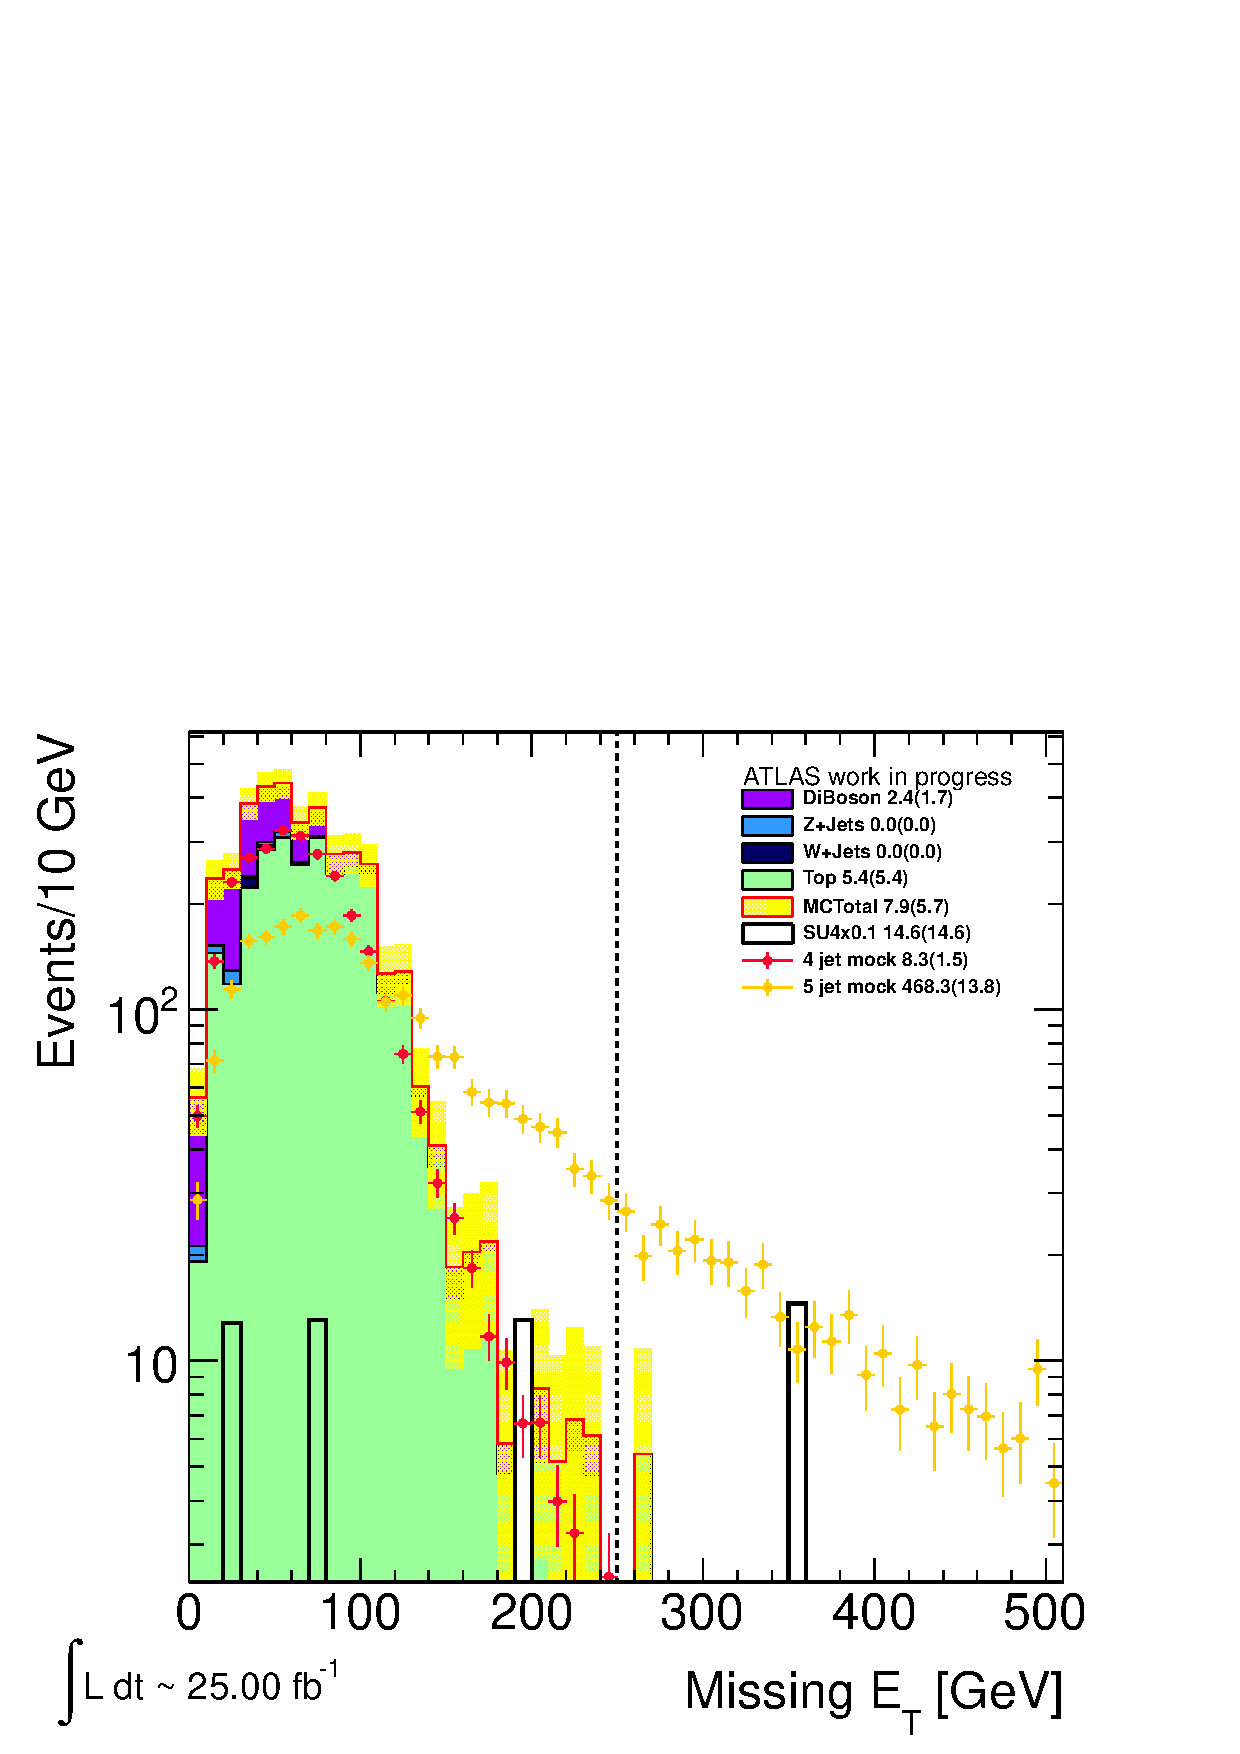
\includegraphics[scale=0.325]{img/Total_OS_ME_etmiss_scaled.pdf}
%     \end{figure}\end{column}
%   \end{columns}
% \end{frame}

% \begin{frame}{Jet pT - different flavour}
%   \begin{columns}
%     \begin{column}{0.5\textwidth}\begin{figure}
%       \caption{$e^{\pm}\mu^{\mp}p_{T}^{\text{jet 1}}$}
%       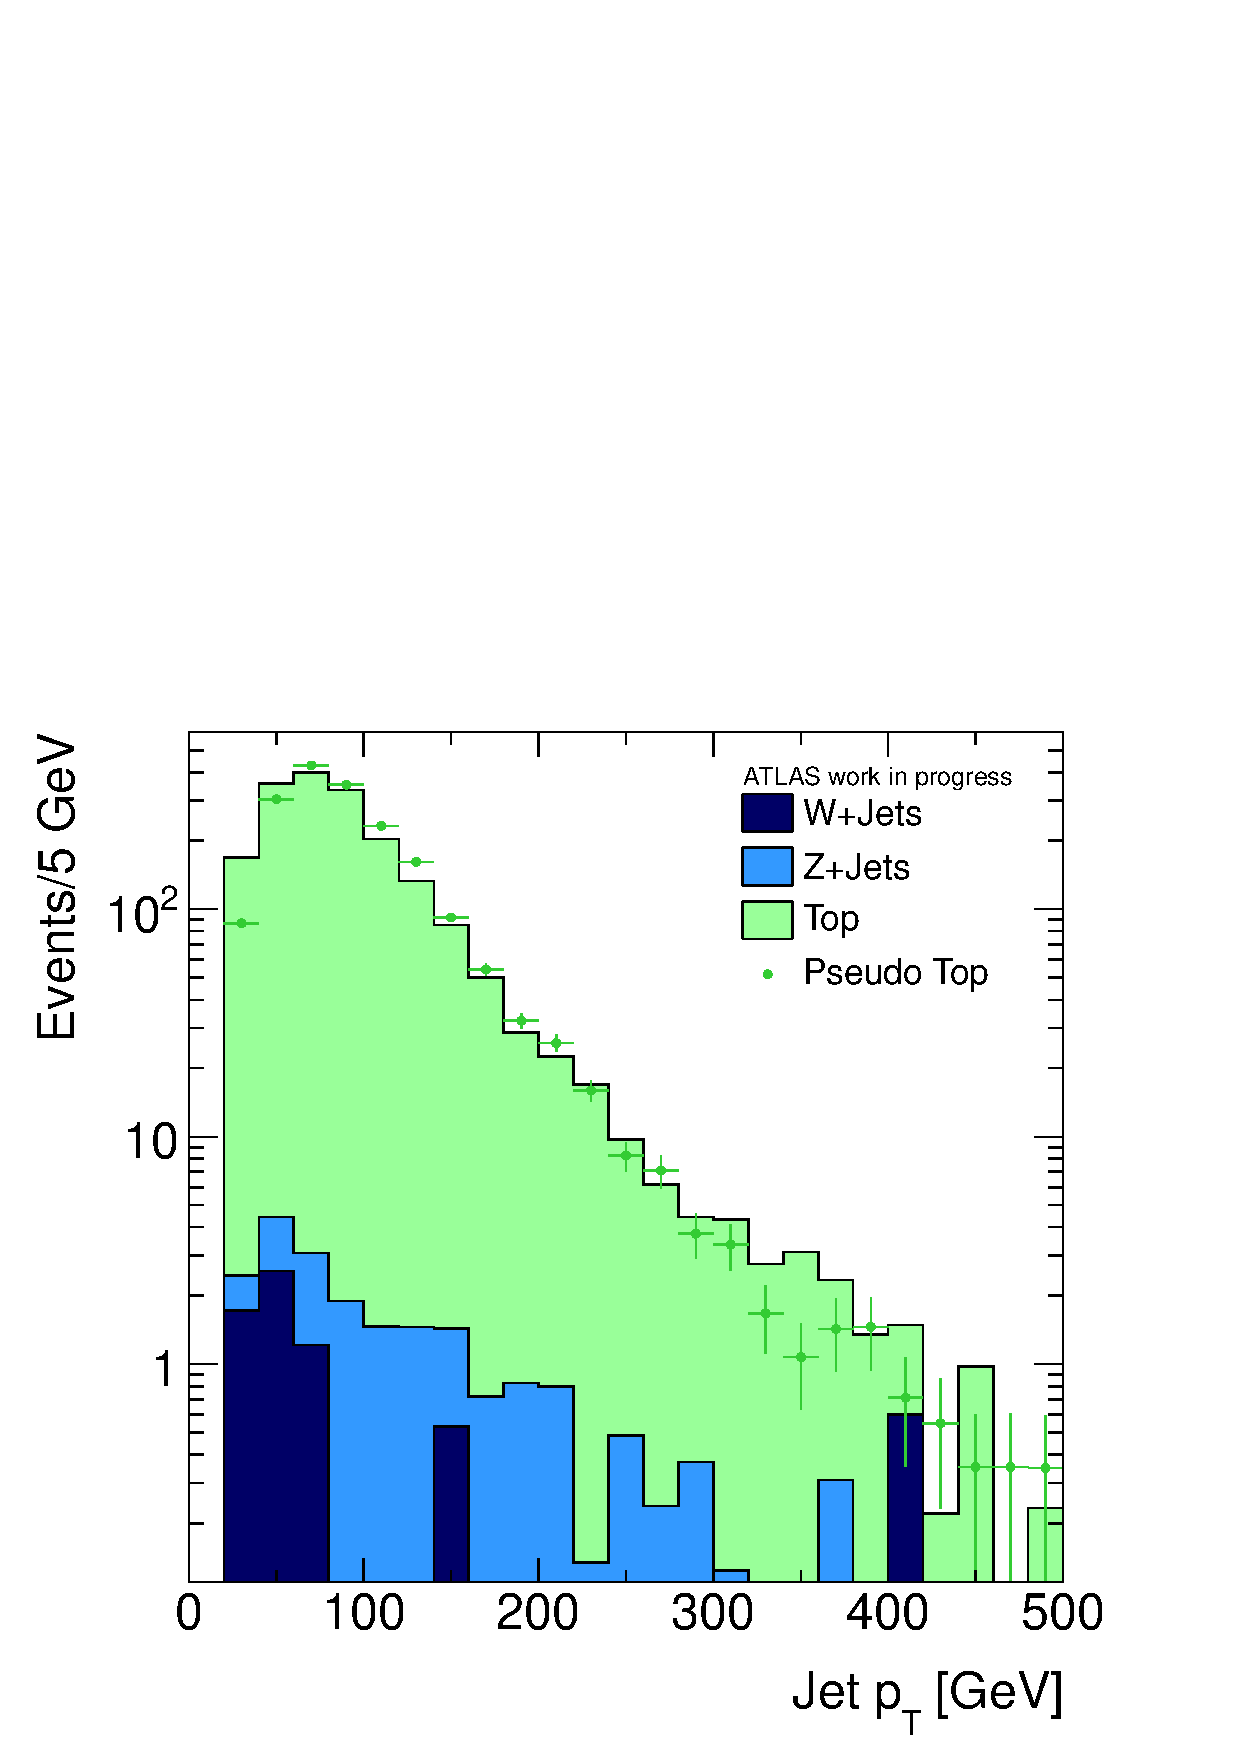
\includegraphics[scale=0.325]{img/Total_OS_EM_jet_lead_pt_scaled.pdf}
%     \end{figure}\end{column}
%     \begin{column}{0.5\textwidth}\begin{figure}
%       \caption{$e^{\pm}\mu^{\mp}p_{T}^{\text{jet 2}}$}
%       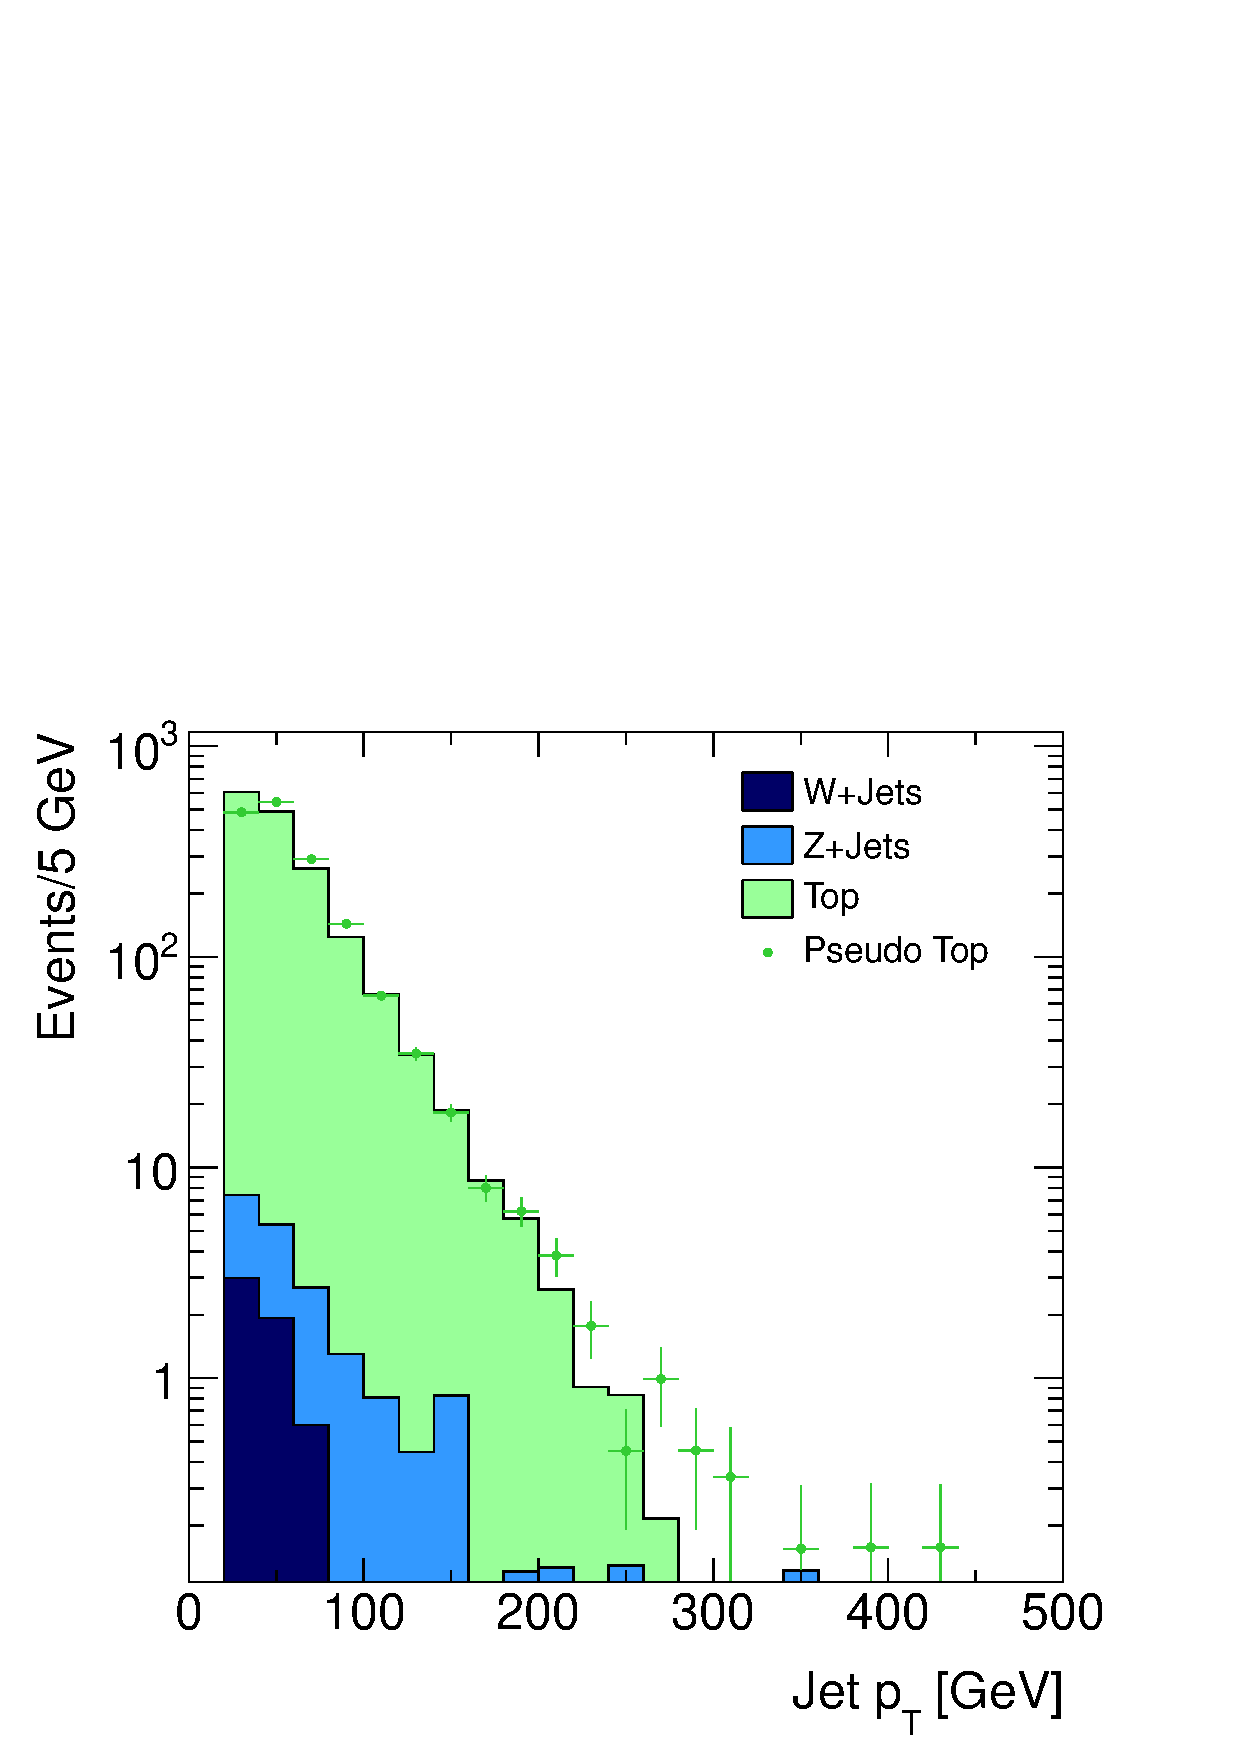
\includegraphics[scale=0.325]{img/Total_OS_EM_jet_lead2_pt_scaled.pdf}
%     \end{figure}\end{column}
%   \end{columns}
% \end{frame}

% \begin{frame}{Jet pT - different flavour}
%   \begin{columns}
%     \begin{column}{0.5\textwidth}\begin{figure}
%       \caption{$\mu{\pm}e^{\mp}p_{T}^{\text{jet 1}}$}
%       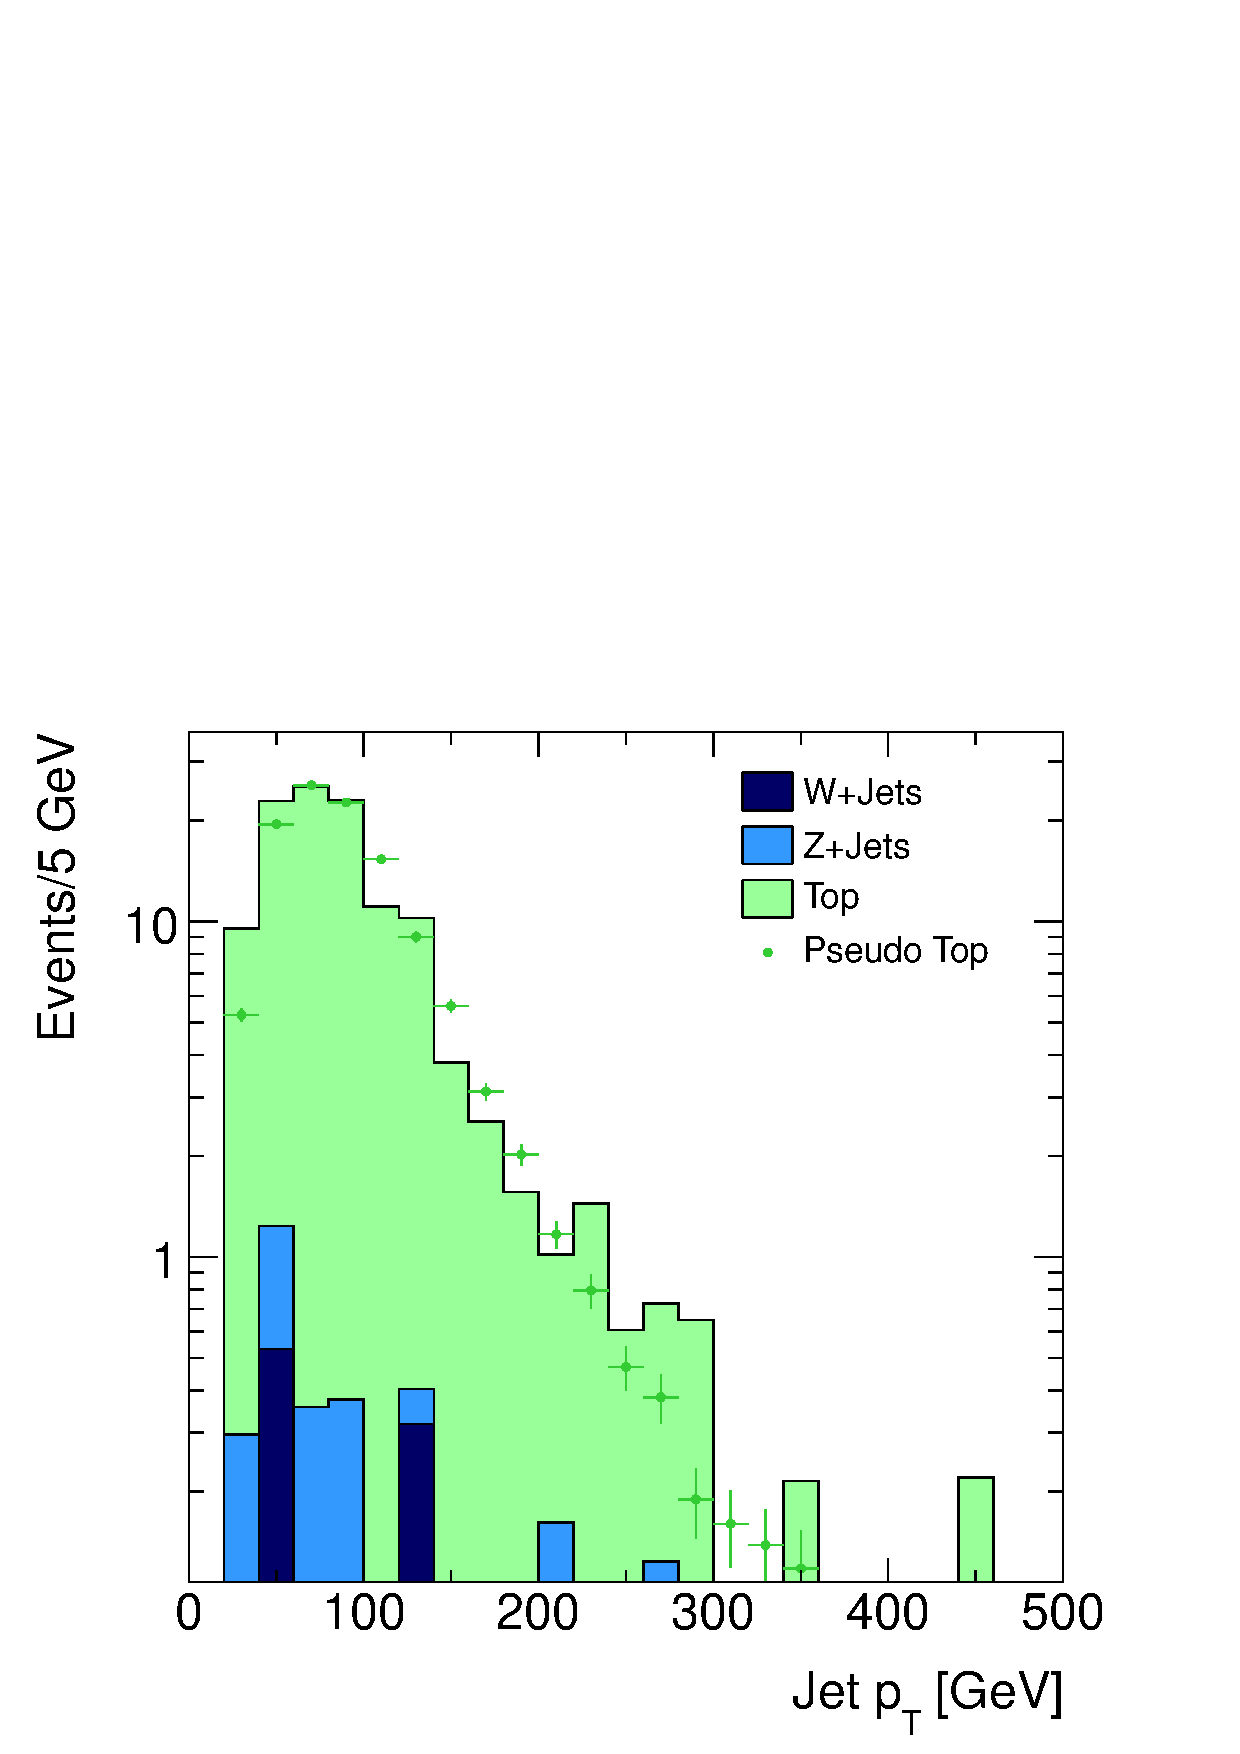
\includegraphics[scale=0.325]{img/Total_OS_ME_jet_lead_pt_scaled.pdf}
%     \end{figure}\end{column}
%     \begin{column}{0.5\textwidth}\begin{figure}
%       \caption{$\mu{\pm}e^{\mp}p_{T}^{\text{jet 2}}$}
%       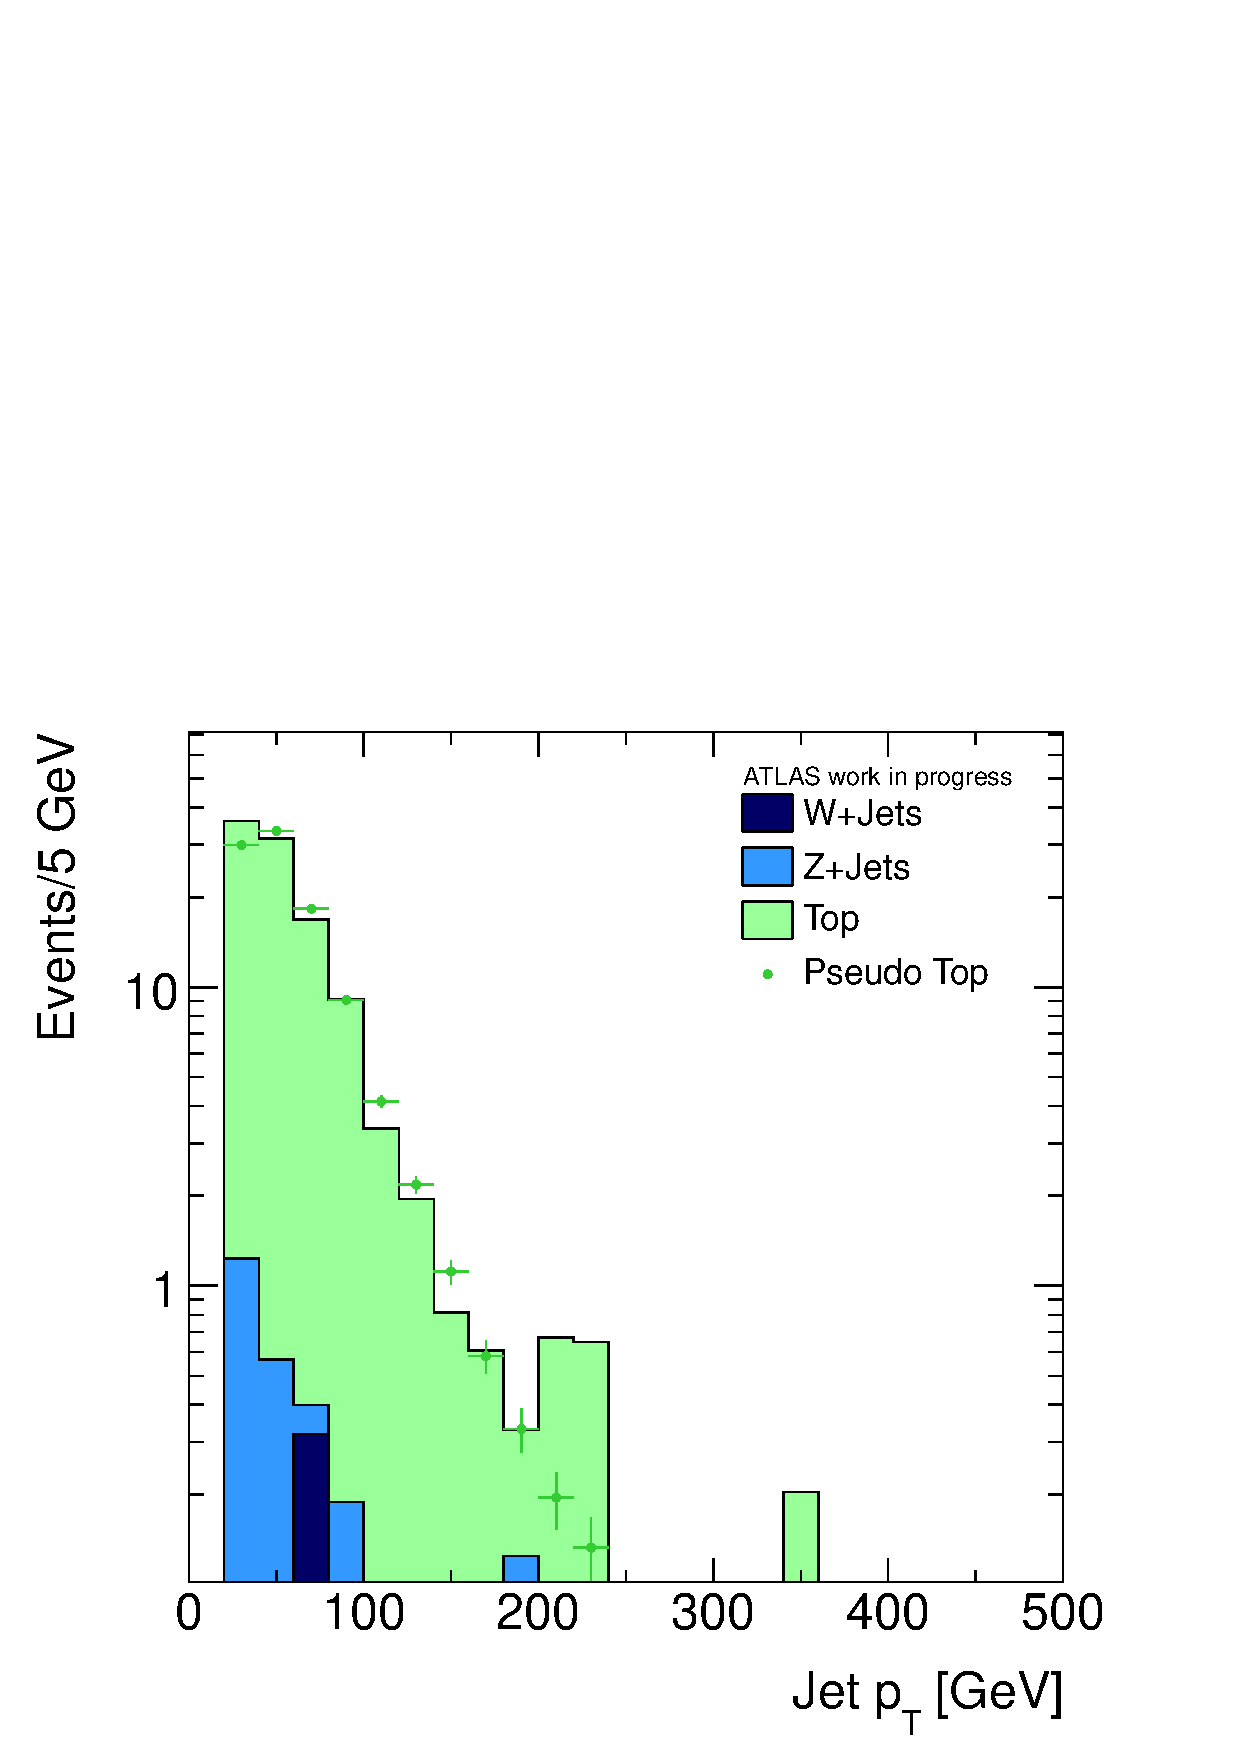
\includegraphics[scale=0.325]{img/Total_OS_ME_jet_lead2_pt_scaled.pdf}
%     \end{figure}\end{column}
%   \end{columns}
% \end{frame}

% \begin{frame}{Jet pT - muons}
%   \begin{columns}
%     \begin{column}{0.5\textwidth}\begin{figure}
%       \caption{$\mu^{+}\mu^{-}p_{T}^{\text{jet 1}}$}
%       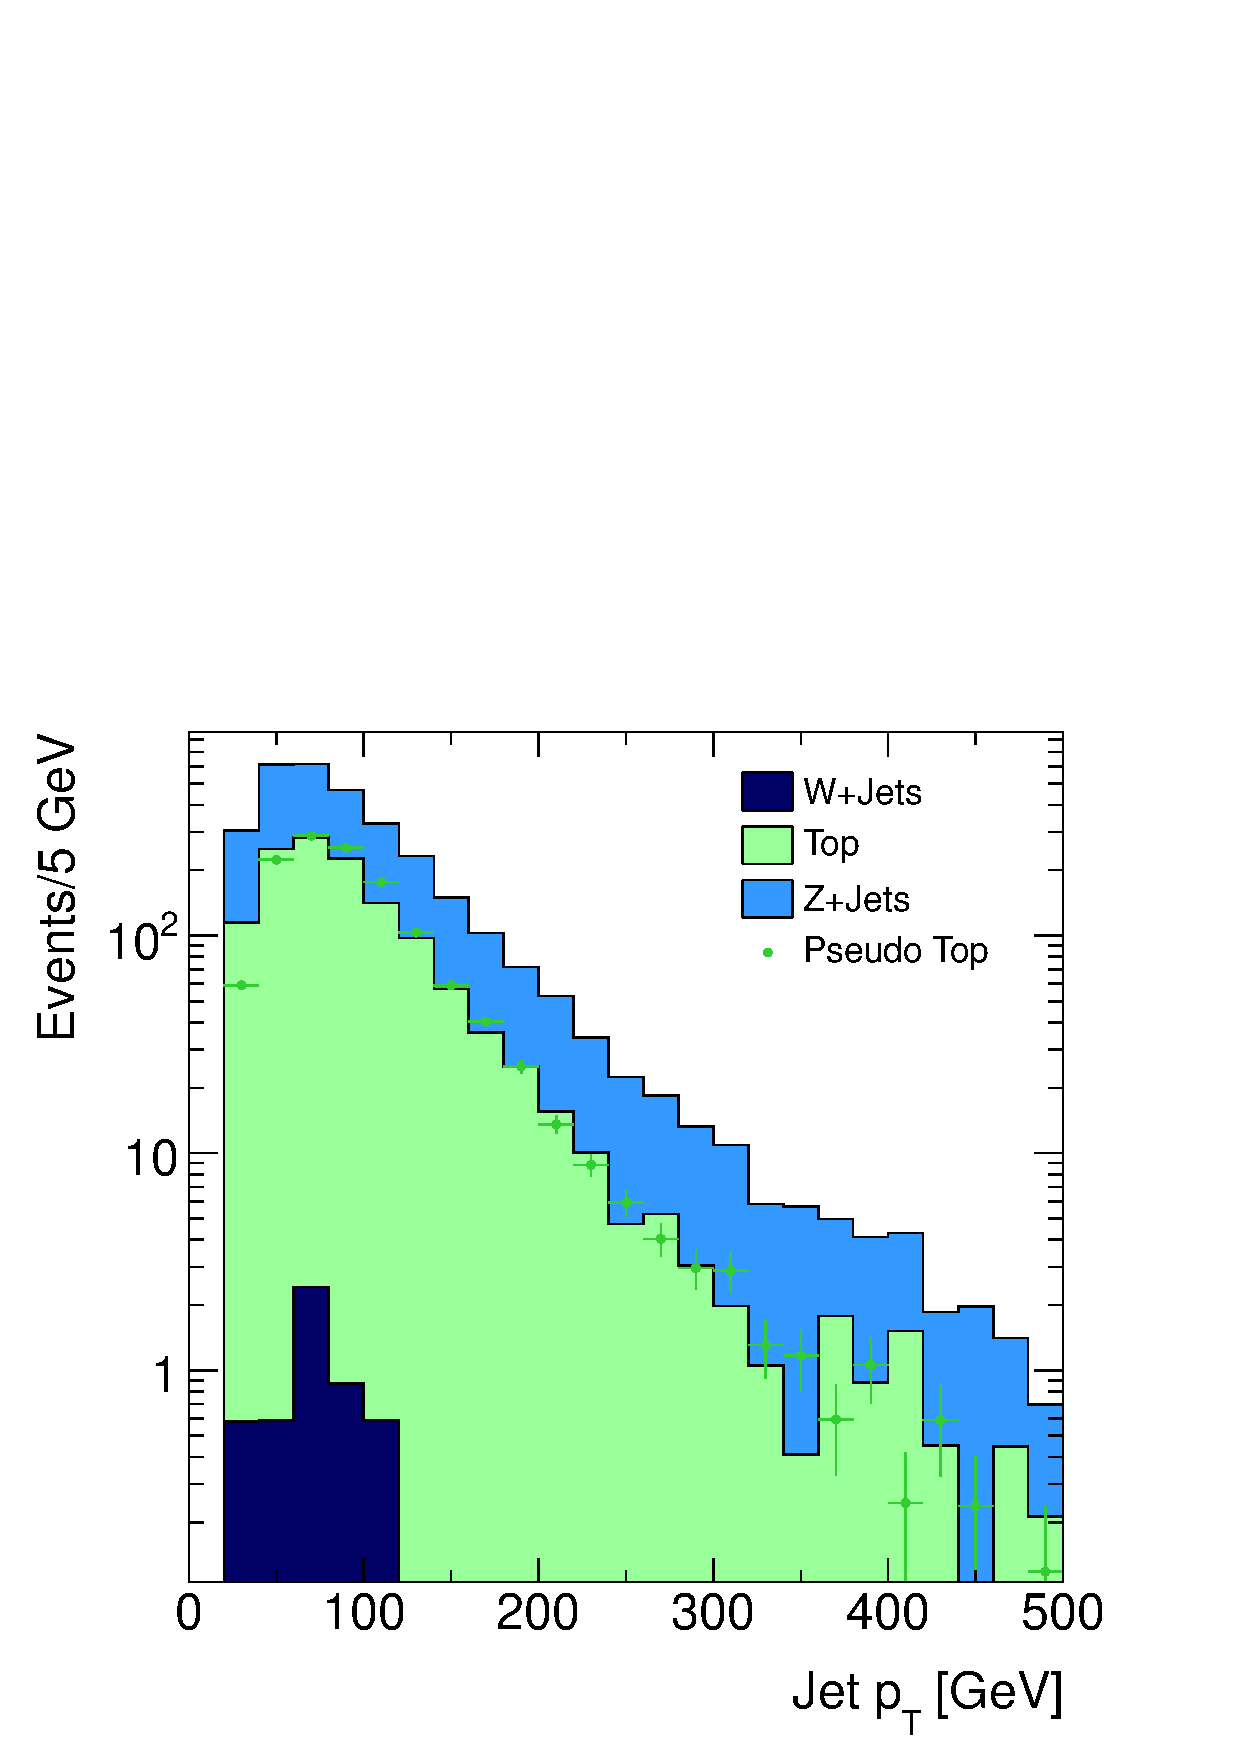
\includegraphics[scale=0.325]{img/Total_OS_MM_jet_lead_pt_scaled.pdf}
%     \end{figure}\end{column}
%     \begin{column}{0.5\textwidth}\begin{figure}
%       \caption{$\mu^{+}\mu^{-}p_{T}^{\text{jet 2}}$}
%       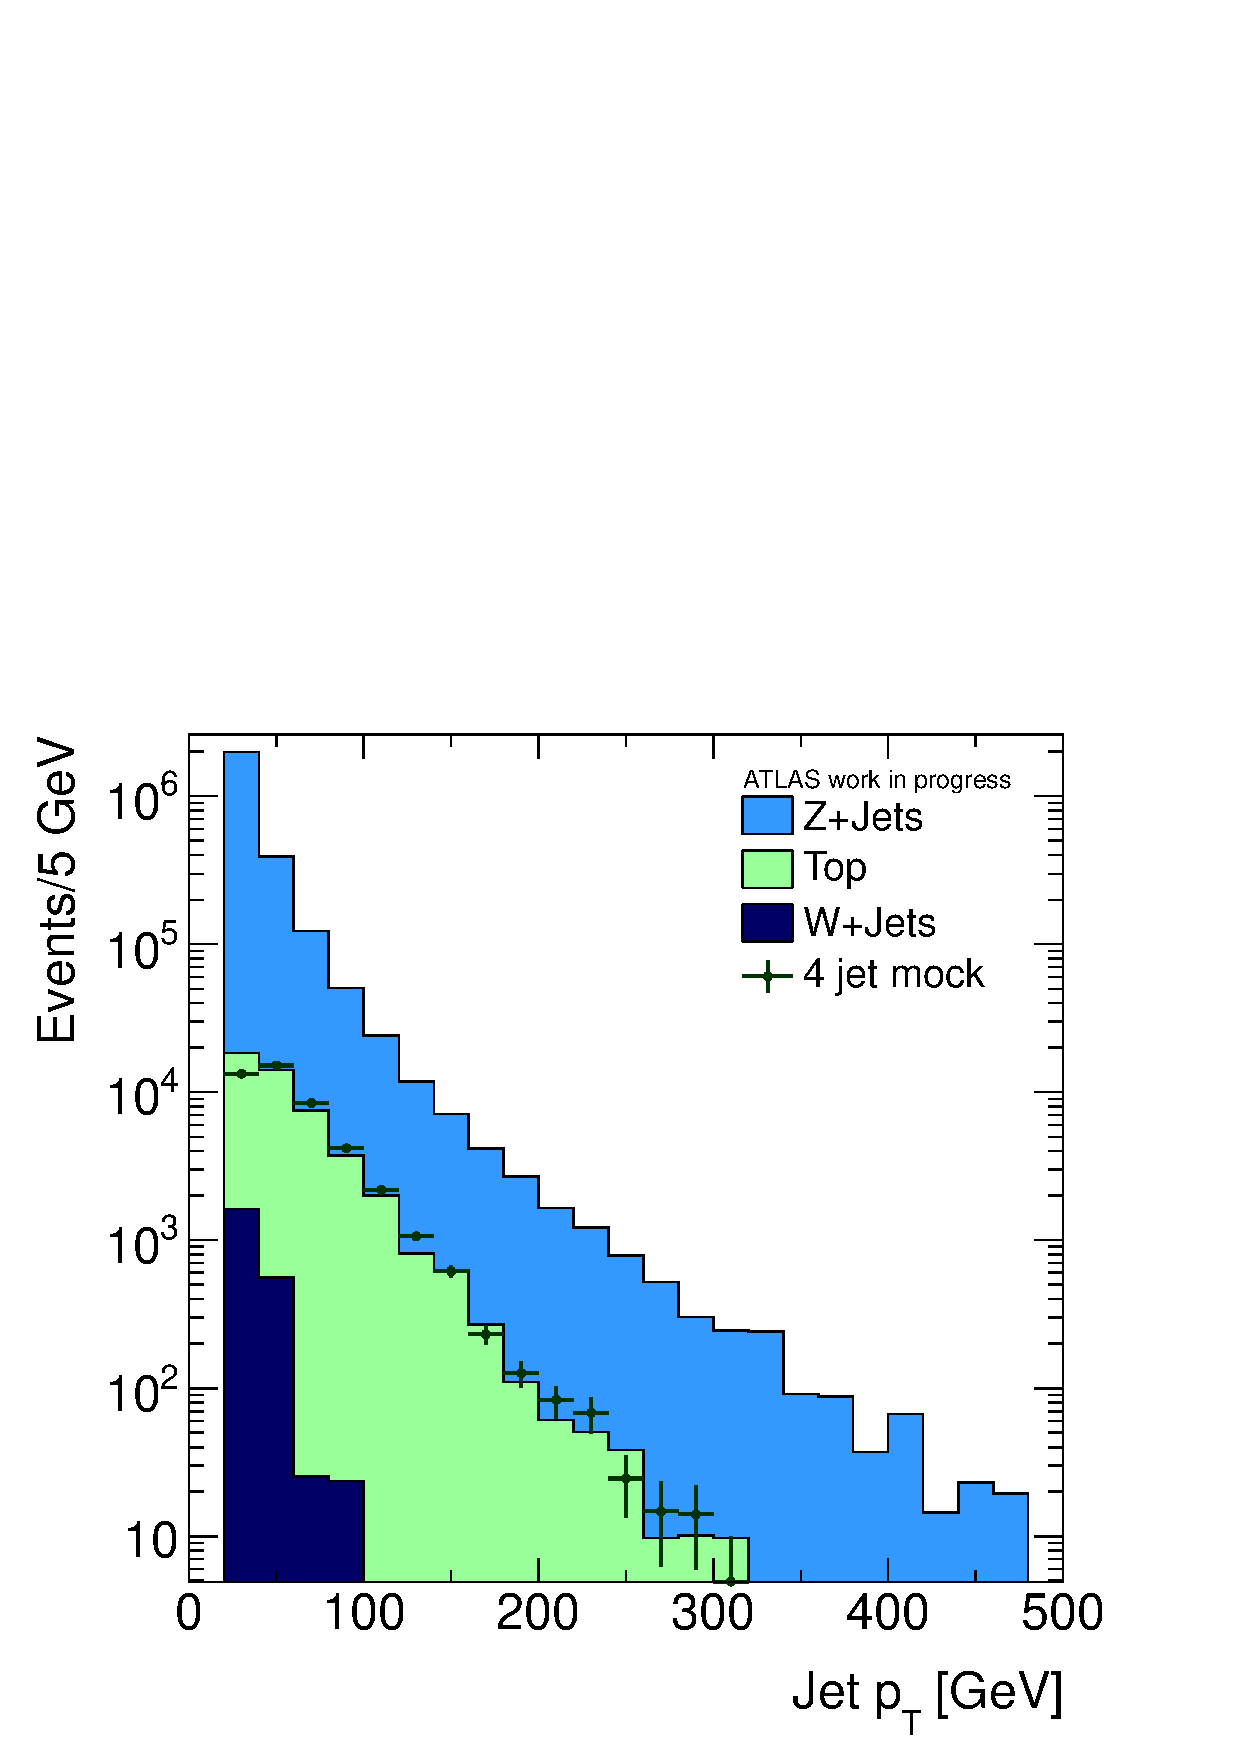
\includegraphics[scale=0.325]{img/Total_OS_MM_jet_lead2_pt_scaled.pdf}
%     \end{figure}\end{column}
%   \end{columns}
% \end{frame}

% \begin{frame}{Partial Chisquare distributions}
%   \begin{columns}
%     \begin{column}{0.5\textwidth}\begin{figure}
%       \caption{$\chi^2_{kinematic}$}
%       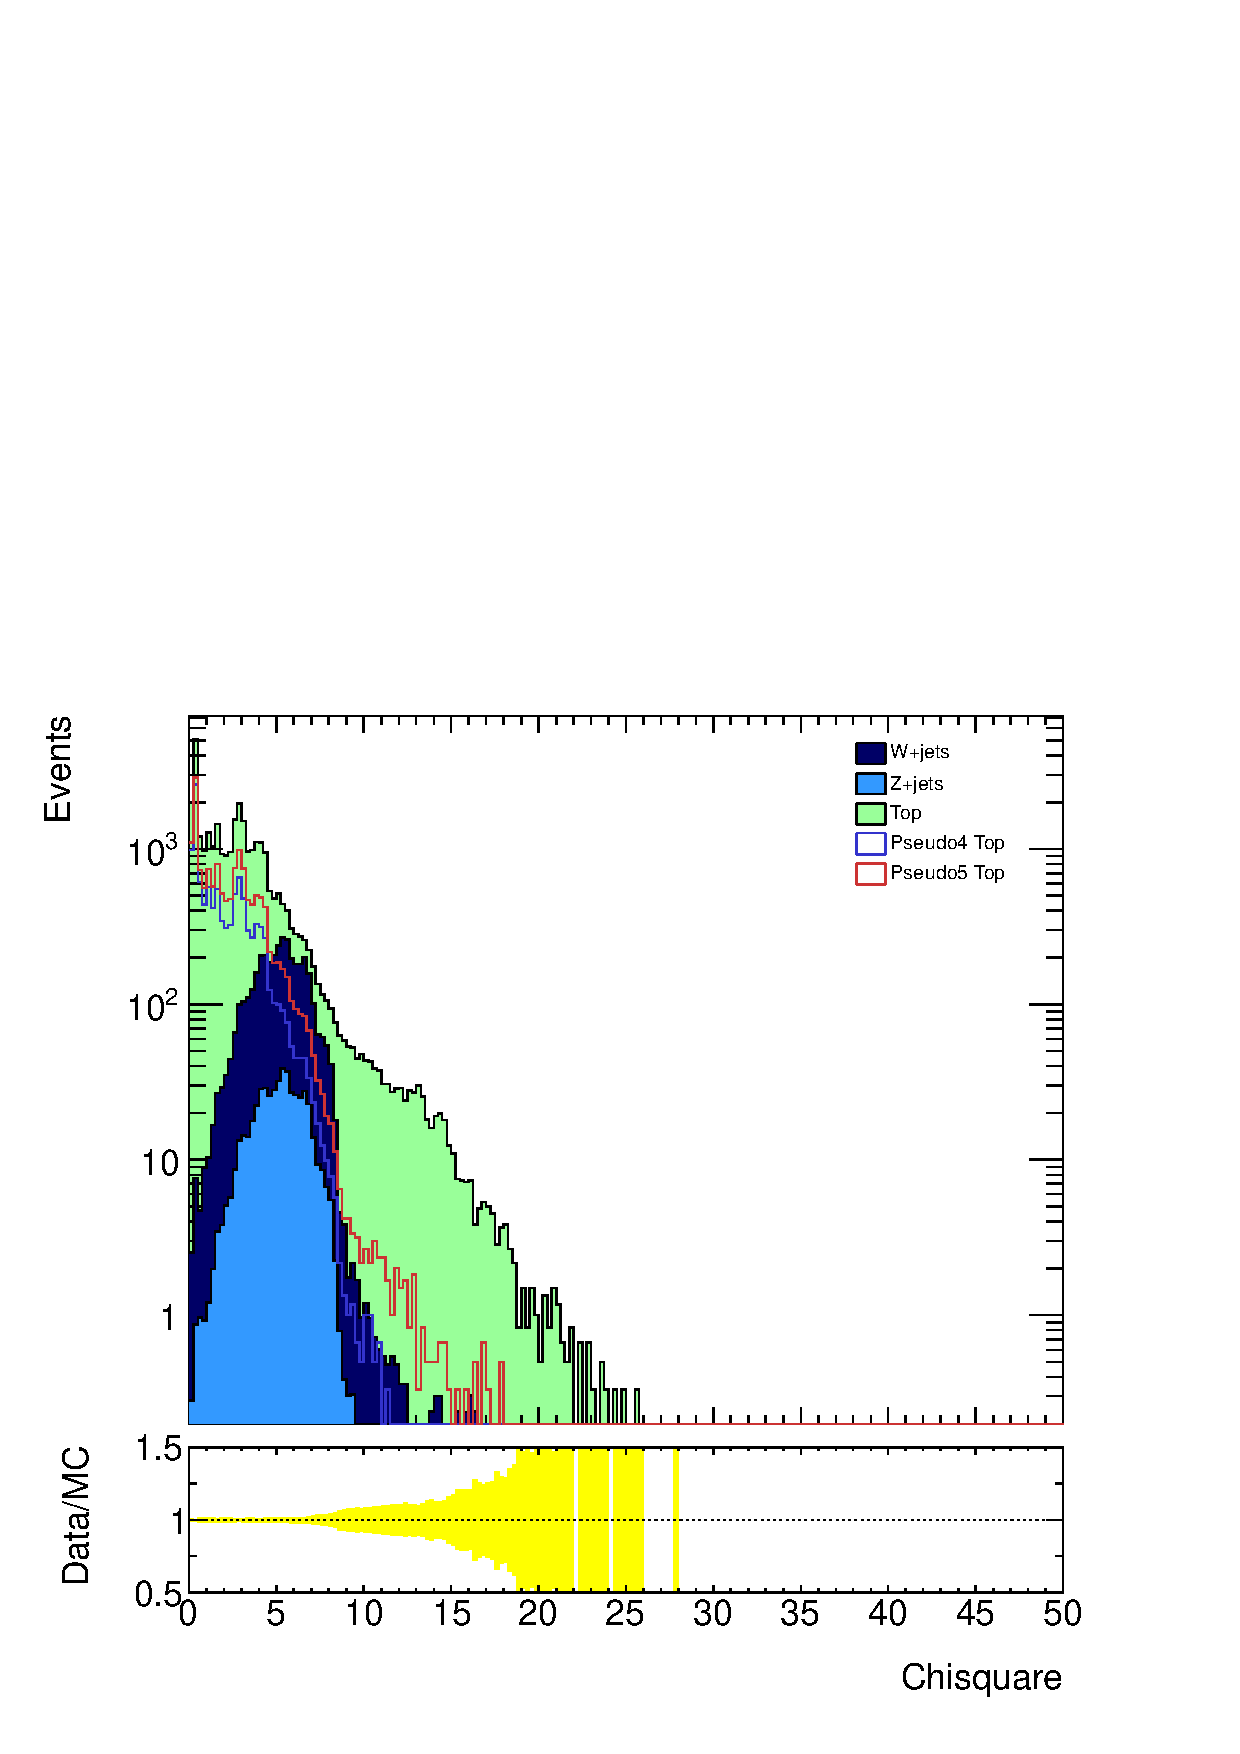
\includegraphics[scale=0.325]{img/Total__min_chi_kin_all4.pdf}
%     \end{figure}\end{column}
%     \begin{column}{0.5\textwidth}\begin{figure}
%       \caption{$\chi^2_{B}$}
%       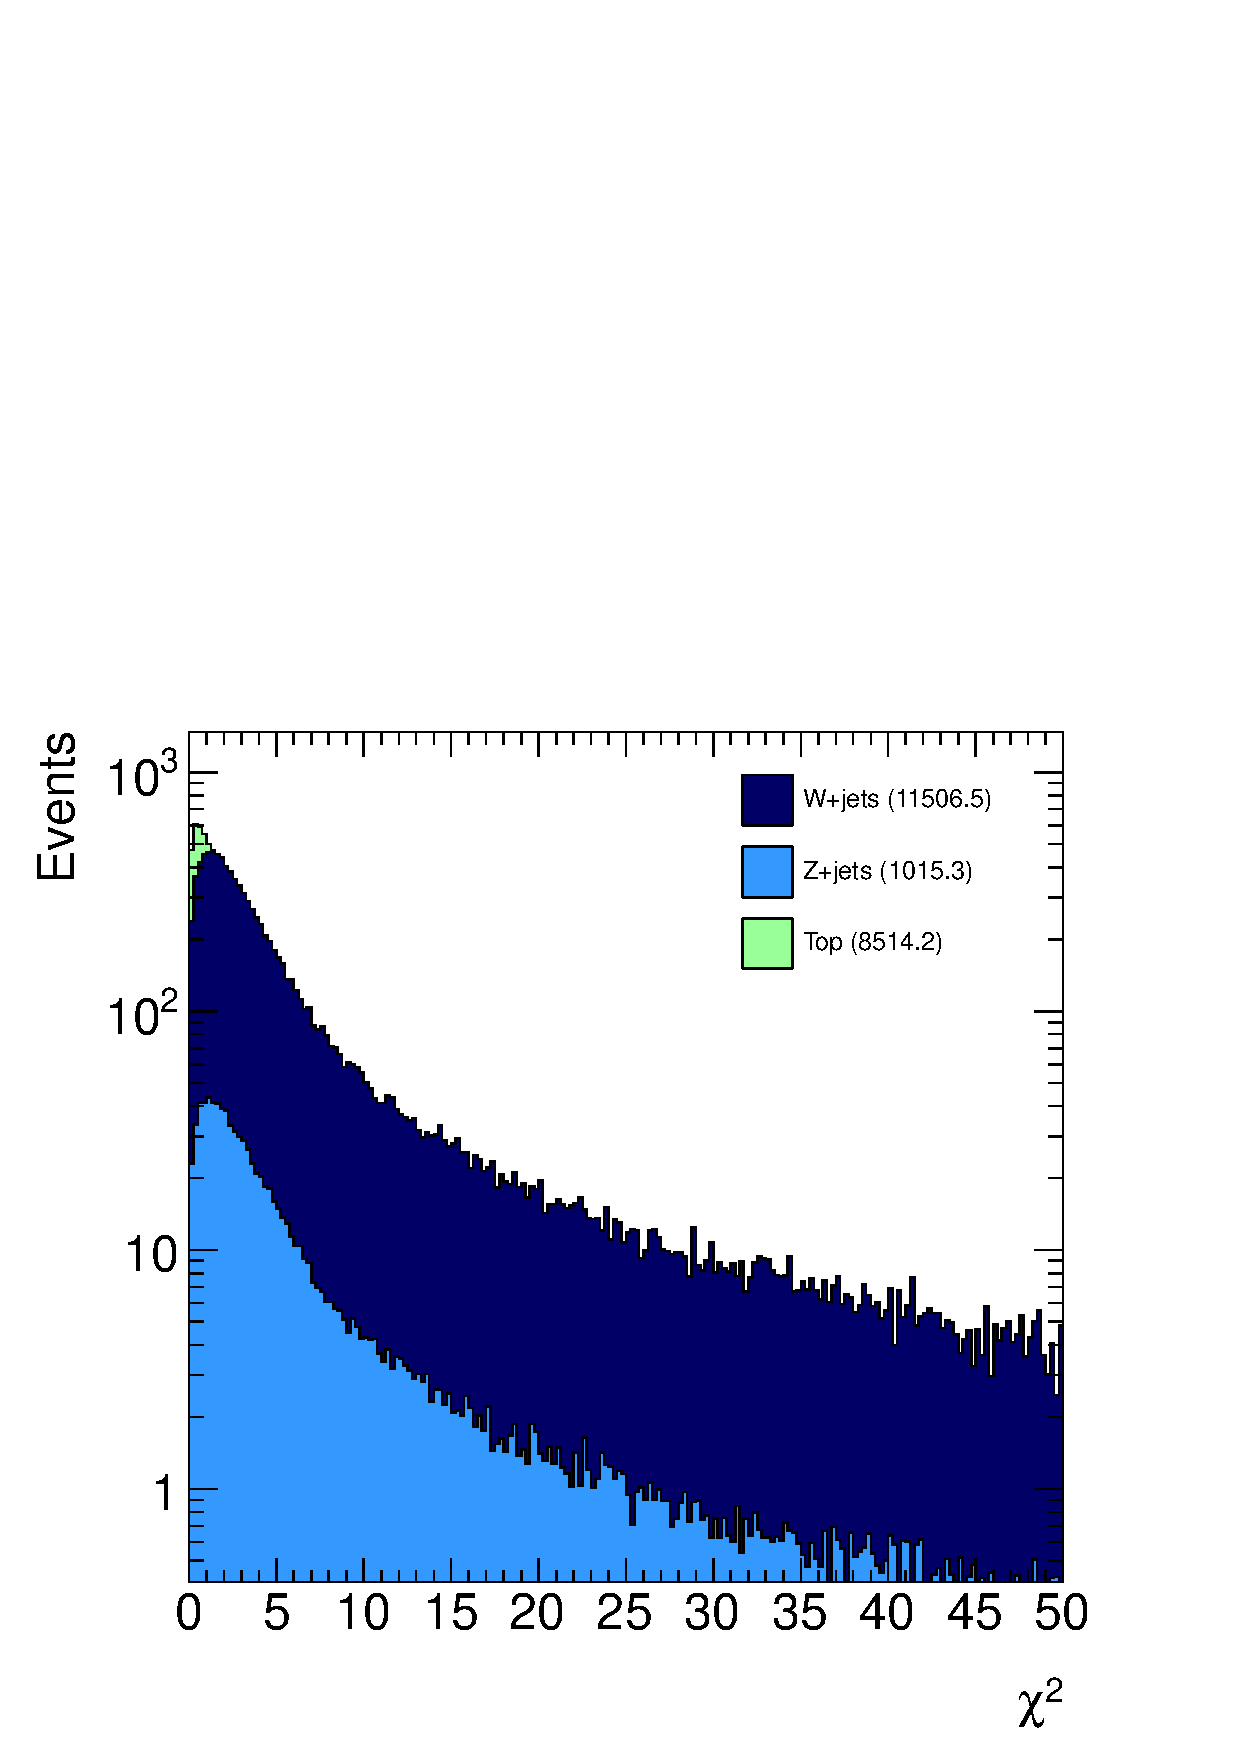
\includegraphics[scale=0.325]{img/Total__min_chi_B_all4.pdf}
%     \end{figure}\end{column}
%   \end{columns}
% \end{frame}

\end{document}
